\documentclass[12pt, a4paper, oneside]{ctexbook}
\usepackage[a4paper, left=3cm, right=3cm, top=2.5cm, bottom=2.5cm]{geometry} % 调整边距
\usepackage{amsmath, amsthm, amssymb, bm, graphicx, hyperref, mathrsfs, fancyhdr, pifont, float, booktabs, longtable}


\title{{\Huge{\textbf{技术经济与工程管理}}}\\——2024秋季学期}
\author{ZZY1234321}
\date{\today}
\linespread{1.5}
\newtheorem{theorem}{定理}[section]
\newtheorem{definition}[theorem]{定义}
\newtheorem{lemma}[theorem]{引理}
\newtheorem{corollary}[theorem]{推论}
\newtheorem{example}[theorem]{例}
\newtheorem{proposition}[theorem]{命题}

\begin{document}

\pagestyle{fancy}
\fancyhf{}
\fancyhead[L]{\leftmark}
\fancyhead[R]{\thepage}
\renewcommand{\headheight}{15pt} % 使用有效的格式
\setlength{\headsep}{20pt} % 设置页眉与正文之间的距离

\maketitle

\pagenumbering{roman}
\setcounter{page}{1}

\begin{center}
    \Huge\textbf{前言}
\end{center}~\

本笔记参考课程老师的PPT,以及b站up主“滹沱河樵夫”发布的“工程经济与管理”合集。如有侵权,可联系本人。笔记解释权归作者本人所有。此笔记正在Github持续更新中,方便的话麻烦点个star,感谢支持。

Github开源链接:https://github.com/ZZY1234321/Course-Notes

如果你是通过付费购买的本笔记,那么恭喜你被骗了,尽快去找那个卖笔记给你的人,看看能不能把钱追回来。

~\\
\begin{flushright}
    \begin{tabular}{c}
        ZZY1234321\\
        \today
    \end{tabular}
\end{flushright}

\newpage
\pagenumbering{Roman}
\setcounter{page}{1}
\tableofcontents
\newpage
\setcounter{page}{1}
\pagenumbering{arabic}

\chapter{绪论}
\section{基本概念}
\subsection{技术(重点)}
是为了满足社会发展需要,运用科学的知识,在改造、控制、协调多种要素的实践活动中创造的劳动手段、工艺方法与技能体系的总称。

\subsection{经济(重点)}
(1)社会生产关系或国民经济的总称。例:工业经济、农业经济等;

(2)社会生产和再生产过程。例:生产、分配、交换、消费等;

(3)经济活动的合理性,即社会劳动的节约、节省或局部生产中的投入产出关系。例:经济效果、经济效益。

注意:《技术经济与工程管理》,此处经济指第3种含义。

\subsection{技术与经济的关系}
相互依赖、相互发展、相互制约。

技术和经济是人类社会物质生产时不可缺少的两个方面,任何一项技术的实施和采用都必须耗用一定的人、财、物,两者既有统一,又有矛盾,既互相联系,又互相制约,既考虑技术进步,先进性,又要考虑经济可行、合理性。

下面有一个简单的题。通过调查研究,设计以下备选方案:
\begin{longtable}{ccc}
\toprule
备选方案 & 学生离学校距离(公里) & 投资额(万元) \\
\midrule
\endfirsthead
\toprule
备选方案 & 学生离学校距离(公里) & 投资额(万元) \\
\midrule
\endhead
\midrule
\multicolumn{3}{r}{{续表}}\\
\endfoot
\bottomrule
\endlastfoot

1. & 1.0 & 6.0 \\
2. & 0.8 & 5.0 \\
3. & 1.2 & 4.4 \\
4. & 2.0 & 3.6 \\
5. & 1.5 & 4.4 \\
\end{longtable}


通过观察以上表格,你首先会排除哪几个方案呢?你最可能选择哪个方案?

这里用到了一种思想,叫做\textbf{帕累托最优}(Pareto Optimality),也称为帕累托效率(Pareto efficiency),是指资源分配的一种理想状态,假定固有的一群人和可分配的资源,从一种分配状态到另一种状态的变化中,在没有使任何人境况变坏的前提下,使得至少一个人变得更好,这就是帕累托改进或帕累托最优化。帕累托最优状态就是不可能再有更多的帕累托改进的余地。

上面一段话可能比较难以理解,我们把它简化一下。帕累托最优解就是,在给定的方案中,如果没有其他的方案在方方面面都比该方案好,那么该方案一定是一个帕累托最优解,即一个非劣解。反之,如果有其他的方案“在方方面面都比该方案好好”或“有些方面比该方案好,有些方面和该方案一样”,那么该方案就不是一个帕累托最优解,即是一个劣解。

在这个例子中,通过比较,可以得出方案1、5为劣解,方案2、3、4为非劣解。

最佳方案的选择(取决于决策者的愿望和倾向性):

(1)如认为就近入学是关键,且费用在4.5万元以下即可,则选方案3;

(2)如认为就近入学是关键,且扩建费用6.0万元以下即可,则选方案2;

(3)如认为扩建费用是关键,即越少越好,则选方案4;

(4)如认为就近入学和扩建费用二者综合考虑,则选方案3。

\subsection{技术经济分析过程}
\begin{figure}[H]
    \centering
    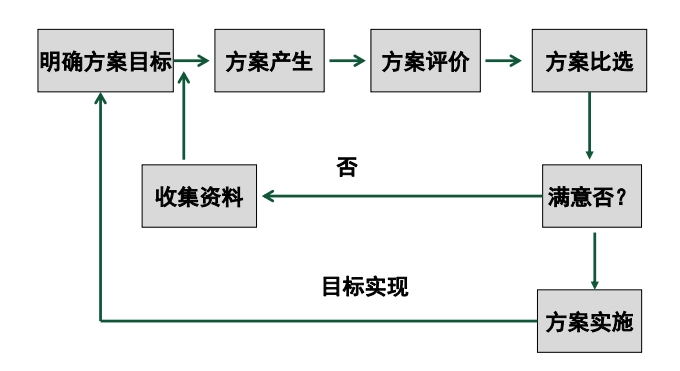
\includegraphics[width=0.8\textwidth]{image/微信截图_20241108214112.png}
    \caption{技术经济分析过程}
    \label{fig:3}
\end{figure}

\textbf{1. 确定目标功能:这是建立方案的基础。}

若我们预计缺30万kw电力,那么我们就要建立一个方案来满足30万kw电力的需要;

若某公司现有3亿元资金寻找投资方向,其目的只有一个:取得较好的回报率,那么我们就要提出一系列投资方案,最终的回报率要达到或超过预期回报率。

\textbf{2. 提出备选方案}

为达到一定目标,必须提出很多方案,如为了解决能源问题可以建火电厂、核电厂或水电站,而建核电站就有许多方案,如采用重水式的、轻水式的……

寻找备选方案,实际上是一项创新活动。人们要求决策者能针对某一特定的问题提出“最优”的解决方法,因而决策者必须创新。

\textbf{3. 方案评价}

方案要经过系统的评价,依据是政策法令与反映决策者意愿的指标体系。如产品要符合国家的产业政策、质量标准;

在符合基本条件后,最重要的是要有较好的经济效益和社会效益。

\textbf{4.选择最优方案}:树立系统观念和动态观念。


\subsection{项目(重点)}
国际项目管理协会(IPMA):项目是\textbf{受时间和成本约束的}、用以实现一系列既定的可交付物(达到项目\textbf{目标}的范围)、同时满足质量标准和需求的\textbf{一次性活动}。

\subsection{项目可行性研究}
项目可行性研究是对项目在投资决策前进行技术经济论证的一门综合性技术。它的任务是\textbf{以市场为前提,以技术为手段,以经济效益为最终目标},对拟建的项目从必要性、可能性、有效性和合理性等方面进行全面、系统地论证,做出项目可行或不可行的评价。

\subsection{财务评价(重点)}
根据国家现行的财税制度和价格体系,在财务效益与费用的估算以及编制财务辅助报表的基础上,编制财务报表,计算财务分析指标,考察和分析项目的\textbf{盈利能力、偿债能力和财务生存能力},判断项目的财务可行性,明确项目对财务主体的价值以及对投资者的贡献,为投资决策、融资决策以及银行贷款等提供依据。

考点1:请你说明什么是盈利能力评价指标,什么是偿债能力评价指标,什么是财务生存能力评价指标。(考察概率小)

答:盈利能力评价指标是用于衡量企业获取利润的能力的指标,反映了企业在一定时期内的收益水平。偿债能力评价指标是指企业偿还各种债务的能力的指标,分为短期偿债能力指标和长期偿债能力指标。财务生存能力评价指标主要是评估企业是否有足够的资金维持正常的生产经营活动,确保企业在一定时期内的资金收支平衡。

考点2:项目财务评价的概念、财务评价重点考查的三种能力是什么?

答:\textbf{盈利能力、偿债能力、财务生存能力}。

考点3:请你说明项目财务评价的作用是什么。

答:考察项目的财务盈利能力;制定项目资金规划的依据;银行发放贷款的重要依据;为协调国家利益和企业利益提供依据。
\chapter{现金流量的构成}
\noindent \textbf{本章知识点:}\\
1.\textbf{现金流入、现金流出}、净现金流量的概念\\
2.\textbf{建设投资}的概念、构成,\textbf{对现金流的影响}\\
3.固定资产、无形资产、其他资产的概念\\
4.固定资产的原值、\textbf{折旧、净残值,折旧对现金流的影响}\\
5.固定资产折旧的方法:\textbf{直线折旧}法、工作量法\\
6.无形资产的\textbf{摊销}\\
7.流动资金投资及其特点、\textbf{对现金流的影响}\\
8.总成本费用的构成\\
9.\textbf{机会成本、沉没成本}\\
10.\textbf{总成本费用和经营成本的区别、联系};二者对现金流的影响\\
11.了解增值税、消费税、企业所得税对现金流的影响\\
12.\textbf{收入、成本、税金和利润的关系}\\
13.区分\textbf{初始现金流、营业现金流及终结现金流}\\
\textbf{注意:加粗部分为期末考试重点内容。}

\section{基本概念}

\subsection{投资}

广义概念:人们的一种有目的的经济行为,即以一定的资源投入某项计划,以获取所期望的报酬。

狭义概念:人们在社会经济活动中为实现某种预定的生产目标而预先垫支的资金。

本课程常用的投资是投资的狭义概念。

包括:\textbf{固定资产投资、流动资金投资、无形资产投资、递延资产投资和预备费用、(建设期利息)}。

固定资产投资活动按其工作内容和实现方式分为:“建筑安装工程”;“设备、工具、器具购置”;“其他费用”三个部分。

\begin{figure}[H]
    \centering
    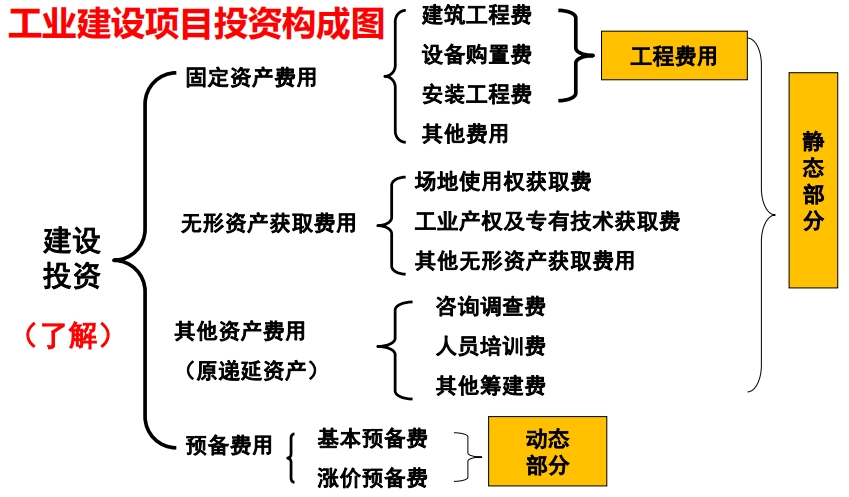
\includegraphics[width=\textwidth]{image/投资分类.png}
    \caption{工业建设项目投资构成图}
\end{figure}

\subsection{现金流量(Cash Flow)}
工业生产活动考察两个方面:物质形态(工具、设备、能耗产品)与货币形态(资金投入、成本收入)。技术经济分析中,把各时点上实际发生的以货币形式体现的资金流出或资金流入称为现金流量。

\subsection{现金流出}
对一个系统而言,凡在某一时点上流出系统的资金或货币量,如投资、费用等。流出系统的现金称为现金流出。(CO)

\subsection{现金流入}
对一个系统而言,凡在某一时点上流入系统的资金或货币量,如销售收入等。流入系统的现金称为现金流入。(CI)

$$
\mbox{净现金流量(}NCF\mbox{)}=\mbox{现金流入(}CI\mbox{)}-\mbox{现金流出(}CO\mbox{)}
$$

现金流量确定原则:收付实现制(实付实收);

会计记账原则:权责发生制(应付应收)。

现金流比会计利润更能反映投资收益,现金流分析是投资决策分析的基础,若现金流预测不准确,无论投资决策分析多准确,都将导致错误的决策。

现金流为投资决策提供重要的价值信息;现金流更有利于考虑资金的时间价值,而会计利润不考虑资金收付时间。

现金流有助于了解收益质量、取得和运用现金的能力,支付本息和股利的能力,同时提供了信用基础。

构成现金流量的基本因素有:成本、投资、税金、利润、收入。\textbf{(往年期中考题)}

\section{各种资产分类}
\subsection{固定资产}
固定资产界定(考点,会考选择题/判断题):

企业为生产商品、提供劳务、出租或经营管理而持有的;\textbf{使用年限超过一个会计年度单位价值较高,并在使用过程中保持原有实物形态的资产}。包括房屋、建筑物、机器、设备等。

\textbf{使用年限要长,单位价值要高,使用过程中要保持原有实物形态的资产(比如煤炭,烧完了就没了,就不算固定资产)。}

\textbf{考固定资产和流动资金的对比或固定资产的三要素。}

以下内容来自百度,但我觉得只要回答出固定资产三要素就可以了,因为这三要素是固定资产的特点:

流动资产是指可以在1年或者超过1年的一个经营周期内变现或者耗用的资产。流动资产投资是指工程在投产前预先垫付、在投产后生产经营过程中周转使用的资金。主要区别为:

〔1〕固定资产投资的结果形成劳动手段,流动资产投资的结果是劳动对象,流动资产投资的数量是由固定资产投资的规模及其结构所决定的。

〔2〕固定资产和流动资产都是生产不可缺少的生产要素,固定资产投资必须有流动资产投资的配合。

〔3〕固定资产投资从工程开工到建成交付使用,往往要经历很长的时间,只有投入没有产出。固定资产投资时间短,回收快。

〔4〕固定资产价值的回收依赖于流动资产的顺利周转。

固定资产计价:原始价值、折旧、净值、重估值、净残值。以下内容将是期末计算题第一题考点:

\subsubsection{固定资产原始价值(原值)}
企业为取得某项固定资产所支付的\textbf{全部价款(包括利息等)}以及使固定资产达到预计可使用状态前所发生的一切合理、必要的支出。包括固定资产费用、固定资产投资借款建设期利息、预备费。

\subsubsection{固定资产折旧}
工业项目投入运营之后,固定资产在使用过程中会逐渐磨损和贬值,其价值逐步转移到产品中去,伴随固定资产损耗发生的价值转移称为折旧。

\subsubsection{固定资产净值}
固定资产使用一段时间后,其原值扣除累计的折旧费总额。
$$\mbox{固定资产原值}-\mbox{累计折旧}=\mbox{固定资产净值}$$

\subsubsection{重估值(重置成本)}
对固定资产按照社会再生产条件和市场情况进行的价值的重新评估。即在当前的生产技术条件下,以现行价格水平重新购建\textbf{同样全新的固定资产}所需要的全部支出。

\subsubsection{预计净残值}
假定固定资产预计使用寿命已满并处于使用\textbf{寿命终了时的预期状态},企业从该项资产的处置中获得的扣除预计处置费用后的金额。

\textbf{折旧是每年都有的,净残值是只有设备最后一年才有的。}
$$\mbox{预计净残值}=\mbox{处置收入}-\mbox{处置费用}$$
或
$$\mbox{预计净残值}=\mbox{固定资产原值} \times \mbox{净残值率}$$
它是固定资产处置时可在市场上实现的价值,对于工业项目的投资者来说,是一项\textbf{在期末可回收的现金流入}。

\noindent \textbf{判断题:}固定资产的残值回收可作为项目的一项现金流入。\\
\textbf{答案:正确}。

\noindent (多选题)下面哪些影响固定资产年折旧额大小?\\
A.固定资产原值大小\\
B.净残值\\
C.折旧年限\\
\textbf{答案:ABC}

这里不讲折旧的计算,在把各种资产分类讲完后统一介绍。

\subsection{流动资产投资}
会计上称为营运资金,营运资本。指在工业项目投产前预先垫付,在投产后的生产经营过程中用于购买原材料、燃料动力,备品备件,支付工资和其他费用,以及在在产品、半成品,产成品和其他存货占用的\textbf{周转资金}。

特点:整个项目寿命期内,流动资金始终被占用且周而复始地流动,到\textbf{项目寿命期结束时},全部流动资金退出生产和流通,以货币资金形式\textbf{回收(现金流入)}。

投产第一年所需的流动资金应在项目投产前安排,为简化计算,项目评价时流动资金可从\textbf{投产第一年}开始安排(\textbf{现金流出})。

储备资金(原材料、燃料等)、生产资金(在制品、半成品、待摊费用)、成品资金(产成品、外购品等)、结算资金(应收、预付帐款等)、货币资金(备用金、现金、银行存款等)。\\
例:(多选)关于流动资金,说法正确的是\\
A.当发生流动资金投资时,应计入现金流出\\
B.一般当寿命期结束时,流动资金作为现金流入\\
C.一般当寿命期结束时,流动资金作为现金流出\\
答案:AB。

\subsection{无形资产}
界定:企业拥有或者控制的没有实物形态的可辨认非货币性资产。如:包括专利、著作权、版权、商标、专有技术、非专利技术、特许权等;其价值在服务期内逐年摊销,摊销费计入成本。

无形资产原值——无形资产购建费用、无形资产投资建设期借款利息;

无形资产的摊销——无形资产的价值在服务期内通过摊销(直线法)的形式计入费用。

\subsection{递延资产}
递延资产,是指本身没有交换价值,不可转让,一经发生就已消耗,但能为企业创造未来收益,并能从未来收益的会计期间抵补的各项支出。包括开办费、租赁固定资产改良费、固定资产装璜、装修费等中在规定年限内平均摊销,摊销费计入成本。

界定:在项目筹建期内实际发生的各项费用,除应计入固定资产和无形资产外的,均计入其他资产(递延资产)。如生产准备费、办公及生活家具购置费等开办费性质的费用直接形成其他资产。

其他资产摊销费——其他资产应在项目投入运营后的一定年限内平均摊销,摊销费计入费用。\\
例1:(多选)建设投资形成的资产包括\\
A.固定资产\\
B.无形资产\\
C.建设期利息\\
D.其他资产\\
答案:ABD。\\
例2:(单选)项目财务评价中确定现金流量的基本原则是\\
A.权责发生制\\
B.收付实现制\\
答案:B。\\
例3:(判断)流动资金投资,当发生时是现金流出,此说法\\
答案:正确。


\section{折旧的计算}
\noindent \textbf{固定资产的折旧方法:}

直线法(年限平均法)

工作量法

双倍余额递减法

年数总和法

\subsection{直线法(使用最广泛)}
$$\mbox{年折旧额}=\mbox{(原值}-\mbox{净残值)}/\mbox{折旧年限}$$
或
$$\mbox{年折旧额}=\mbox{固定资产原值} \times \mbox{年折旧率}$$
$$\mbox{年折旧率}=(1-\mbox{净残值率})/\mbox{折旧年限}×100\%$$

例题1:某固定资产原值为1万元,预计净残值率为4\%,折旧年限为5年,则按平均年限法计算年折旧率、年折旧额及第3年末帐面净值分别为多少?

解:$f=\frac{1-4\%}{5} \times 100\% = 19.2\%$

$D=10000 \times 19.2\%=1920$(元)

$K_3=10000-1920 \times 3=4240$(元)


\subsection{工作量法}
(1)计算公式
$$\mbox{单位工作量折旧额=(固定资产原值-净残值)/预计使用年限内可完成的工作量}$$
$$\mbox{年折旧额=单位工作量折旧额} \times \mbox{年实际完成的工作量}$$
(2)特点

使用年限内每年的单位折旧额不变,年折旧额随年实际工作量而变化。

(3)适用-某些专业设备、交通运输车辆等。

例题2:计算一台估计生产10万个单位的设备折旧额。设备成本为1万元,预计前两年每年生产2万个单位,第三年生产3万个单位,第四年生产1万个单位,最后一年生产2万个单位。

解:不给净残值时,净残值默认为0。

单位产量折旧额$=(10000-0)/100000=0.1$(元)

第一年折旧额$=0.1 \times 20000 = 2000$(元)

第二年折旧额$=0.1 \times 20000 = 2000$(元)

第三年折旧额$=0.1 \times 30000 = 3000$(元)

第四年折旧额$=0.1 \times 10000 = 1000$(元)

第五年折旧额$=0.1 \times 20000 = 2000$(元)

\subsection{双倍余额递减法}
(1)含义(看不懂就去看公式和例题)

在寿命期 1 到(n - 2)年,不考虑固定资产残值的情况下,根据每期期初固定资产账面净值和双倍的直线法折旧率计算固定资产折旧。

在寿命期的最后两年,将第 n - 1 年年初的固定资产账面净值扣除净残值后的余额进行平摊。

\textbf{刚开始折旧多,后面折旧少。前期可以少交税。}

(2)计算公式(记住就行)

1 到 n - 2 年:
$$\mbox{年折旧率=}2 / \mbox{折旧年限} \times 100\%$$
$$\mbox{年折旧额=每年年初固定资产账面净值} \times \mbox{年折旧率}$$
第 n - 1 年、第 n 年:
$$\mbox{第 n - 1 年年初固定资产账面净值-净残值} /2$$

例题3:仍以例题1数据为例,双倍余额递减法的年折旧率$=2/5=0.4$,各年折旧额及年末帐面净值如下表所示(从第四年起改为直线折旧)。
\begin{table}[H]
\centering
\caption{双倍余额递减法折旧计算表}
\begin{tabular}{cccc}
\toprule
使用年限 & 年折旧率 & 年折旧额(元) & 年末净值(元) \\
\midrule
0 & 0 & 0 & 10000 \\
1 & 0.4 & 4000 & 6000 \\
2 & 0.4 & 2400 & 3600 \\
3 & 0.4 & 1440 & 2160 \\
4 &  & 880 & 1280 \\
5 &  & 880 & 400 \\
\bottomrule
\end{tabular}
\end{table}

\subsection{年数总和法}
(1)计算公式(了解一下吧,感觉不会考)
$$\mbox{年折旧率}=\frac{(\mbox{折旧年限}-\mbox{已使用年限)}}{[\mbox{折旧年限} \times (\mbox{折旧年限}+1)\div 2]}$$
$$\mbox{年折旧额}=(\mbox{原值}-\mbox{净残值}) \times \mbox{当年折旧率}$$
其中,折旧年限指预计总使用年限,已使用年限按照每年年初算;净残值计算时,每年计提折旧的基数不变,但是乘当年折旧率时,每年折旧率减少。

(2)特点

年折旧率和年折旧额都逐年减少,前期可以少交税。

例题4:仍以例题1数据为例,按年数总和法计算的各年折旧率、年折旧额及年末帐面净值如下表所示。
\begin{table}[H]
\centering
\caption{年数总和法折旧计算表}
\begin{tabular}{cccc}
\toprule
使用年限 & 年折旧率 & 年折旧额(元) & 年末净值(元) \\
\midrule
0 & 0 & 0 & 10000 \\
1 & 5/15 & 3200 & 6800 \\
2 & 4/15 & 2560 & 4240 \\
3 & 3/15 & 1920 & 2320 \\
4 & 2/15 & 1280 & 1040 \\
5 & 1/15 & 640 & 400 \\
\bottomrule
\end{tabular}
\end{table}

\subsection{总结}
注意:这里的点可能会考选择题,最后一点可考计算。

采用不同的折旧方法,对同一资产来说,计提的\textbf{折旧总额是相同的},只是每年计提的折旧数额不同;

无形资产、其他资产(原递延资产)的摊销与固定资产折旧的性质相同,均是把固定资产、无形资产、其他资产(原递延资产)的原始价值在一定期限内采用一定的人为方法进行分摊。

计提的折旧数额、摊销数额均计入产品成本或当期费用,即固定资产、无形资产、递延资产的价值通过计提折旧、摊销的方式转移到产品成本中,或转化为当期的费用。

在进行现金流量分析时,\textbf{计提折旧与摊销既不发生现金的流入,也没有发生现金流出},但因其\textbf{计入了成本费用},因而会\textbf{影响当期的利润数额}。

折旧和摊销虽然不是现金流入和流出,但是因为它影响了利润,所以会进而影响到税金。

\noindent \textbf{自测题(不要翻看前面的内容,直接作答):}

\noindent 1. (单选)对同一资产来说,采用不同的折旧方法:\\
A. 计提的折旧总额是相同的,只是每年计提的折旧数额不同。\\
B. 计提的折旧总额不相同的,每年计提的折旧数额也不同。\\
C. 计提的折旧总额是相同的,每年计提的折旧数额也相同。\\
D. 计提的折旧总额是不同的,每年计提的折旧数额相同。

\noindent 2. (单选)在进行现金流量分析时,计提折旧与摊销:\\
A. 不发生现金的流入,但会发生现金流出。\\
B. 发生现金的流入,但不发生现金流出。\\
C. 既不发生现金的流入,也不发生现金流出。\\
D. 既发生现金的流入,也发生现金流出。

\noindent 3. (单选)关于折旧,说法正确的是\\
A. 折旧不影响成本费用的大小\\
B. 折旧不影响现金流量\\
C. 折旧有的时候是现金流出\\
D. 折旧总额的大小不受折旧年限的影响\\
\textbf{答案:A、C、D。}

\section{费用、成本}
\subsection{概念解释}
费用:企业在生产经营过程中发生的各项耗费。(针对一定时间期间)

成本:企业为生产产品和提供劳务所发生的各项费用。(针对产品或劳务)

总成本费用:指项目在一定时期内(一般为一年)为生产和销售产品而花费的全部成本和费用。
\subsection{成本的分类}
成本计算范围:总成本费用、单位产品成本。

财务评价要求:总成本费用、经营成本。

成本与产量:固定成本、可变成本。

其他方式:机会成本、资金成本等。

\subsection{总成本费用的构成——按经济用途分类(看看,有个印象就行)}
\begin{figure}[H]
    \centering
    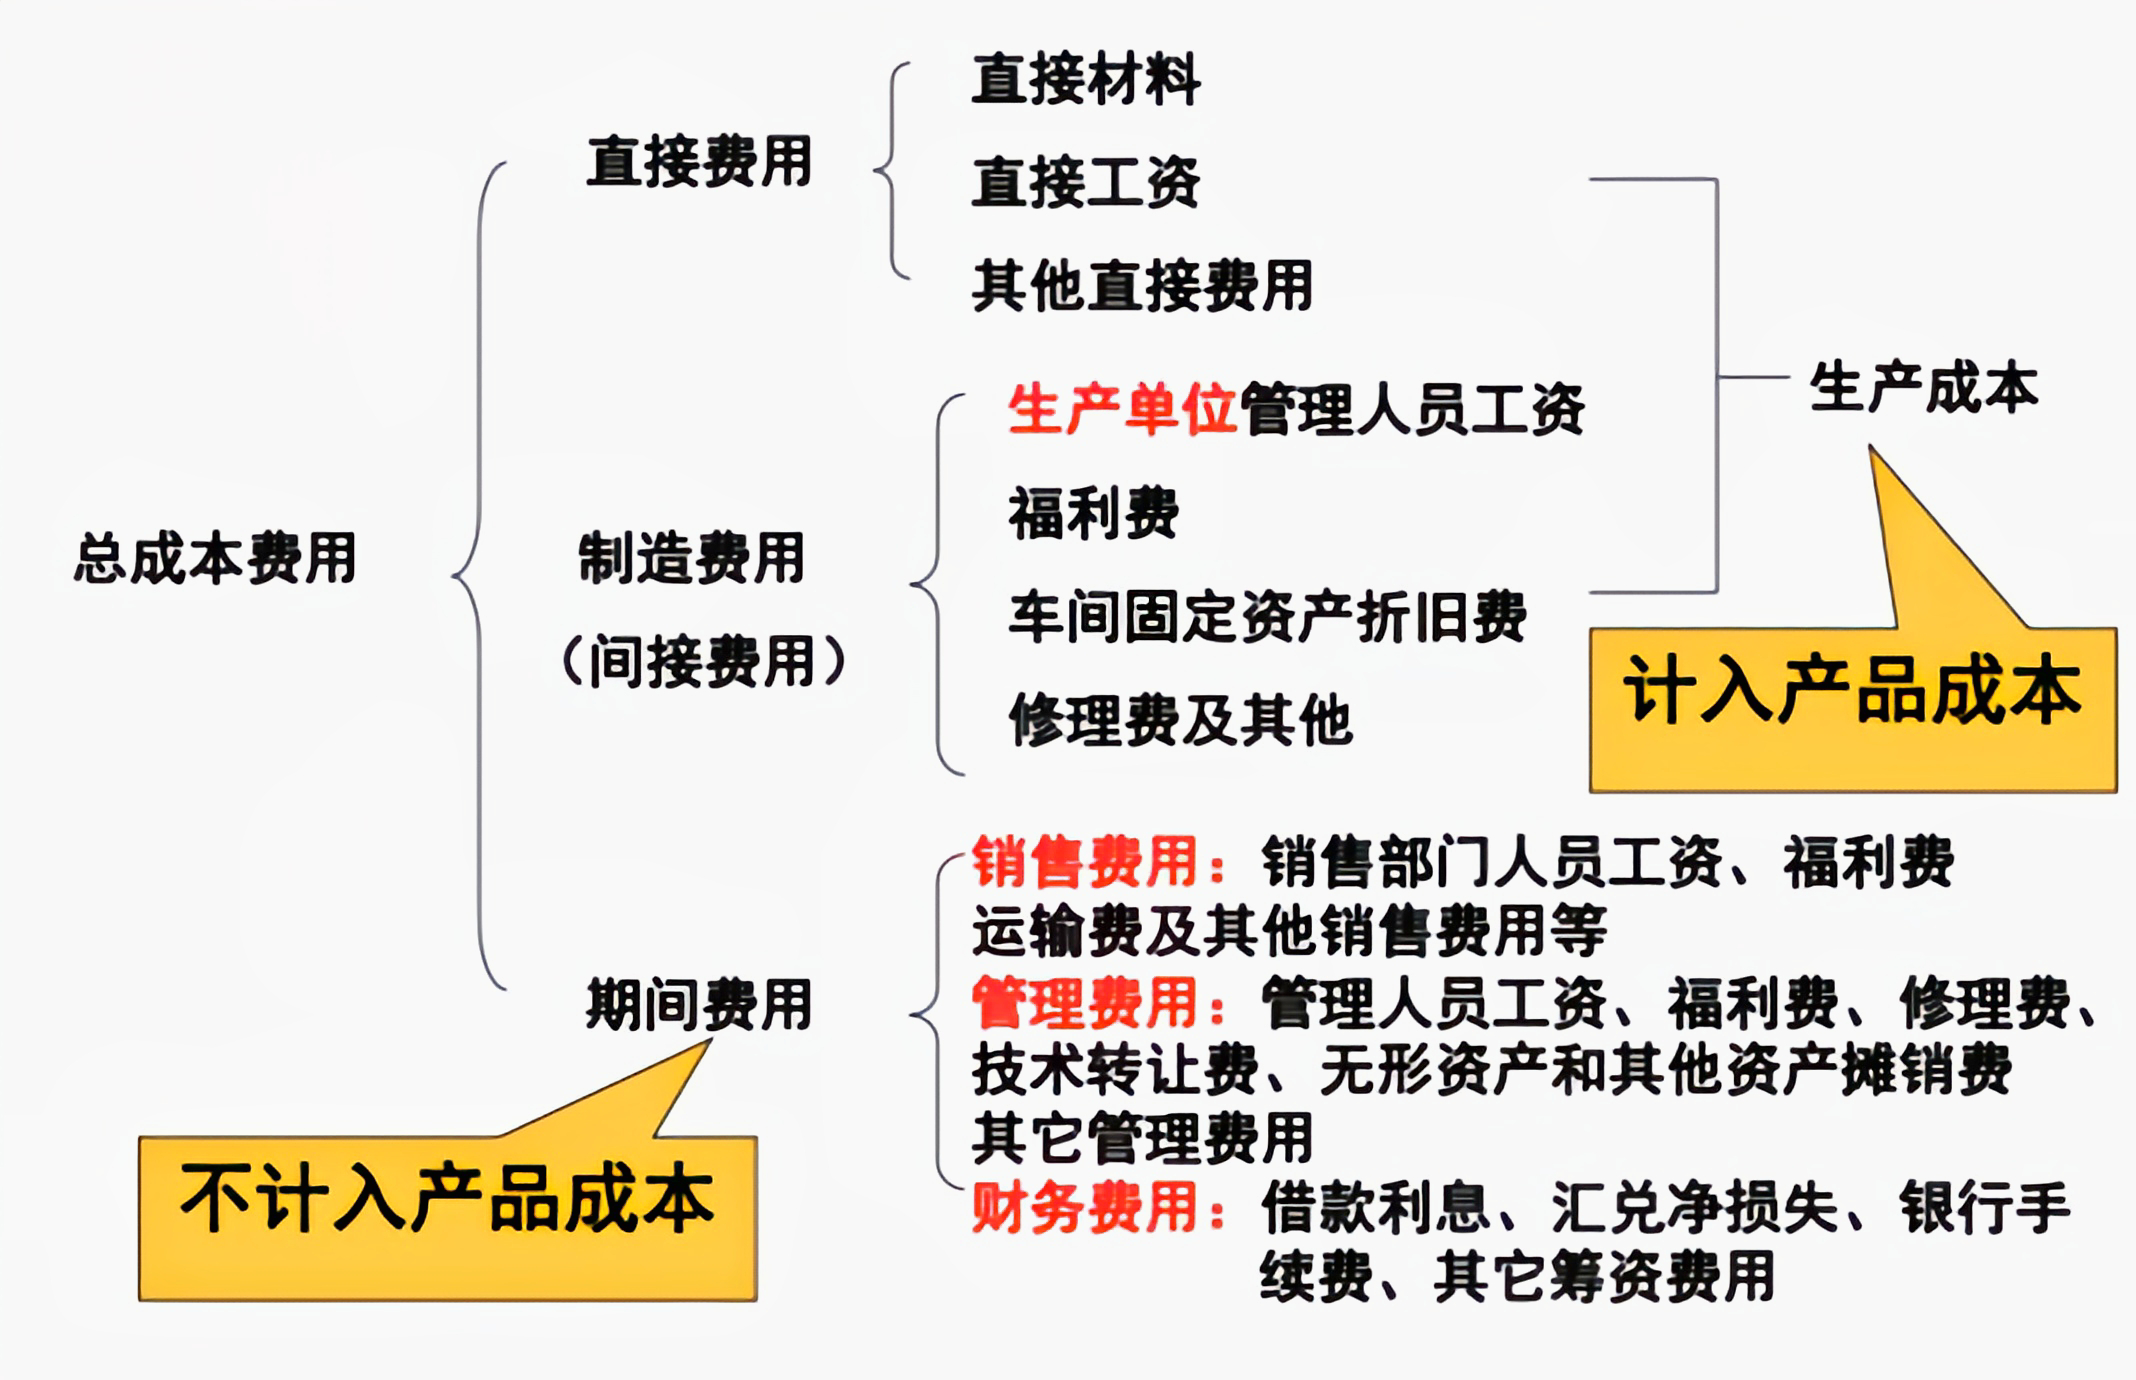
\includegraphics[width=\textwidth]{image/总成本费用构成.png}
    \caption{总成本费用构成图}
\end{figure}

\textbf{(1)直接费用}

直接材料:用于产品生产、构成产品实体的材料的消耗;

直接工资:生产产品的工人工资;

其他直接费用:生产产品的工人福利费、产品生产过程中燃料动力的消耗。

\textbf{(2)制造费用(间接费用)}

界定:生产单位为组织和管理生产所发生的各项间接费用;

举例:生产单位(车间或分厂)管理人员工资、福利生产单位固定资产折旧费、修理费,及其他制造费用(办公、差旅、劳保费等);

直接费用和相应的制造费用,称为产品生产成本;

已销售产品的生产成本,称为产品销售成本。

\textbf{(3)期间费用(不计入产品成本的费用)}

销售费用:商品销售过程中发生的费用,运输、装卸、包装、保险、广告宣传费、专设销售机构的费用等。

管理费用:企业行政管理部门为管理和组织经营活动而发生的各项费用。如管理部门人员工资及福利、折旧、无形资产的摊销、办公费、修理费等;

财务费用:企业在筹集资金等财务活动中发生的费用,包括利息支出、汇兑净损失、银行手续费等。

\subsection{总成本费用构成-按表现形态分类(看看,有个印象就行)}
按照表现形态分类,总成本费用包括:外购材料(原材料、辅料、半成品、包装物、备件、低耗品等)、外购燃料、外购动力、工资+福利费、折旧费、摊销费、利息支出、修理、其他(税金)。

\subsection{技术经济分析中有关成本费用的概念}
(1)技术经济分析中对成本、费用的理解与企业财务会计中的理解不完全相同:

(2)会计中的成本和费用是对企业生产经营过程中实际已经发生的各种耗费的真实、唯一的记录;

(3)技术经济分析中使用的成本和费用数据是在一定假设前提下对拟实施投资方案的未来情况预测的结果,带有不确定性;

(4)会计中对费用和成本的计量是分别针对特定会计期间和特定产品生产过程;

(5)技术经济分析中对费用和成本的计量则一般是针对某一投资项目或技术方案的实施结果;

(6)技术经济对成本、费用的分析,强调对现金流量的影响分析,一般不严格区分成本、费用概念;

(7)技术经济分析中还需引入会计中不使用的一些成本概念。

\textbf{例1:}(判断题)技术经济分析中使用的成本和费用数据是企业生产经营过程中实际已经发生的各种耗费的真实、唯一的记录。

\textbf{答案:}错误。

\textbf{例2:}某公司拟新建车间,需要使用公司现在拥有的一块土地,在进行投资分析时,因为公司不必动用资金去购置土地,应该将该土地的成本考虑在内吗?

\textbf{答案:}应该考虑,这属于\textbf{机会成本}。以下是具体解析。

土地的成本应考虑在内,因为该公司若不利用这块土地兴建车间,则它可将这块土地移作他用,并取得一定的收入。只是现在由于在这块土地上兴建车间才放弃了这笔收入,而这笔收入代表兴建车间使用土地的机会成本。

假设这块土地出售可净得15万元(假设此为该土地所有可能获取收益中最高的收益),它就是兴建车间的机会成本。

Tips:不管该公司当初是以5万元还是20万元购进这块土地,都应以现行市价作为这块土地的机会成本。

\subsection{机会成本}
上个例题引入了一个新的概念,机会成本。这个是需要理解并掌握的。

\subsubsection{涵义:}
机会成本是指将一种具有多种用途的有限资源置于某种特定的用途,而放弃的用于其他各种用途的最高收益。

机会成本的概念来源于这样的现实:资源是稀缺的。资源的稀缺性决定了人类只有充分考虑了某种资源用于其他用途的潜在收益后,才能作出正确的决策使有限的资源得到最佳、有效的利用。

\subsubsection{意义:}
机会成本不是一种实际发生的支出或费用,而是失去的收益,这种收益不是实际发生的,而是潜在的。\textbf{它在会计记录中是没有的。}

在决策中,机会成本有利于人们全面考虑可能采取的各种方案,以便为特定、稀缺资源寻求最为有利的使用途径。在技术经济分析中,\textbf{机会成本会影响现金流量。}

\textbf{例1:}企业有一台机多用床,可以自用,也可以出租,出租可以获得7000元的年净收益,自用可以产生6000元的年净收益。

1. 当舍弃出租方案而采用自用方案时,其机会成本为 [填空1] ,其利益为 [填空2] ;

2. 当舍弃自用方案而采用出租方案时,其机会成本为 [填空3] ,利益为 [填空4] 。

\textbf{答案:}7000元;-1000元;6000元;1000元。

\textbf{例2:}某公司在2017年曾经打算新建一个车间,并请一家公司作过可行性分析,支付咨询费5万元。后来由于各种原因该项目被搁置下来。 2019年旧事重提,在进行投资分析时,这笔咨询费是否需要考虑呢?

\textbf{答案:}不需要。这属于\textbf{沉没成本}。无论是否进行投资,这笔支出都不会改变。

\subsection{沉没成本}
那么上题就引入了新概念,沉没成本。需要理解,但不是重点。
\subsubsection{涵义:}
沉没成本是指过去已经支出的,与当前决策无关的成本。
\subsubsection{意义:}
它对企业决策不起作用,它主要表现为过去发生的事情,费用已经支付,今后的任何决策都不能取消这项支出。

如果将沉没成本纳入投资方案的总成本,则一个有利的方案可能因此变得不利,从而造成决策错误。\\
\textbf{例题:}(单选)在项目投资中,下列哪一个因素不应该考虑\\
A. 现金流入\\
B. 机会成本\\
C. 沉没成本\\
D. 资金成本\\
\textbf{答案:}C。

\subsection{经营成本/付现成本}
此部分需要\textbf{理解并掌握}。

\subsubsection{引入:}
在技术经济分析中,需要考察投资项目的现金流入与现金流出。按照会计核算的方法,总成本费用中含有既不属于现金流入也不属于现金流出的\textbf{折旧和摊销费}。

建设投资中有固定资产投资和无形资产投资部分,已作为现金流出,总成本费用中又有对固定资产和无形资产的按期计提的折旧和摊销,若再作为流出,等于多流出一次,故要计算项目各年实际发生的现金流出,\textbf{必须从总成本费用中将折旧费和摊销费剔除。}

\textbf{即经营成本是为了经济分析方便,从总成本费用中分离出来的与投资分摊、资金筹措无关的一部分费用。}

计算:

经营成本=总成本费用-折旧费-摊销费-\textbf{借款利息支出}

注意:

技术经济分析中通常将“经营成本”作为一个单独的现金流出项;

如果分析中需要考虑借款利息支出,则另列一个现金流出项。

\noindent \textbf{例题:}(多选)下列说法错误的是\\
A. 机会成本任何时候都不影响现金流量\\
B. 经营成本是现金流出\\
C. 总成本费用是现金流出\\
D. 沉没成本不影响项目未来的现金流\\
\textbf{答案:}AC。

\section{营业收入}
\textbf{涵义:}通过销售产品、提供劳务等取得的货币收入。

\textbf{作用:}是技术经济分析中现金流入的重要组成部分;

\textbf{计算:}销售收入=商品销量 × 商品销售单价(以市场价格计算)

\section{税金}
\subsection{概念(了解即可)}
税收:国家为了实现其职能、凭借政治权力,按法律规定的标准,强制地、无偿地取得财政收入的一种特定的分配形式。

税金:国家依据法律对有纳税义务的单位和个人征收的财政资金。

作用:积累财政资金,进行宏观调控。

\textbf{税金和费用的区别:}
费用是政府机关为单位或居民个人提供服务或授予国家资源和资金的使用权而收取的代价,遵循\textbf{有偿}原则。

\subsection{税金的分类-按性质和作用分类(了解)}
\textbf{(1)流转税类:}

以商品生产、流通和劳动服务的流转额为征税对象。

内容:增值税、消费税。

\textbf{(2)所得税类:}

以法人或个人的纯所得为征税对象的各种税。

内容:企业所得税、个人所得税。

\textbf{(3)资源税类:}

以被开发或占用的资源为征税对象的各种税。

内容:资源税、土地使用税。

\textbf{(4)财产税类:}

以法人或自然人拥有及转移的财产价值或增值额为征税对象的各种税。

内容:房产税、车船使用税、土地增值税。

\textbf{(5)特定目的税类:}

国家为达到某种特定目的而设立的各种税。

内容:城市维护建设税、车辆购置税、印花税等。

\textbf{(6)关税}

主要对进出我国国境的货物、物品征收。

内容:关税。

\subsection{主要税种的涵义、纳税金额的计算}
重点:\textbf{增值税}、消费税、城市维护建设税、教育费附加、\textbf{企业所得税}等。

\subsubsection{(1)增值税}
\textbf{征收对象:}增值税是对在我国境内销售货物或提供加工、修理修配劳务以及进口货物的单位和个人征收的一种税。\textbf{增值税是价外税。}增值税不影响最后利润。

\textbf{应纳税额的计算(一般纳税人)}

计算公式为:

应纳税额=当期销项税额-当期进项税额

销项税额=销售额(销售时销售方收取)×增值税税率(0,6\%,9\%,13\%)

进项税额=购买价款(购买时购买方支付)×增值税税率(0,6\%,9\%,13\%)

\textbf{增值税的流程:}
\begin{figure}[H]
    \centering
    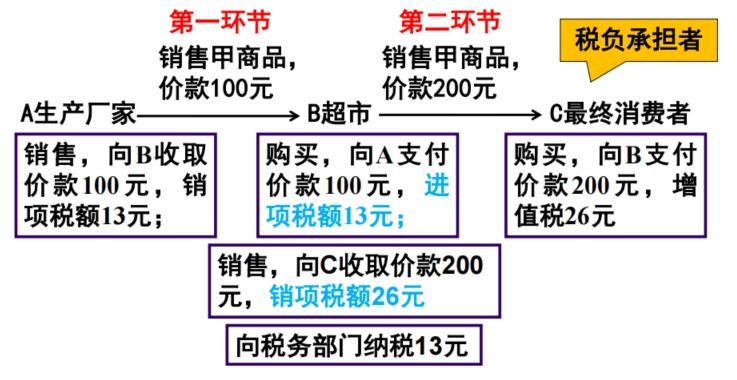
\includegraphics[width=\textwidth]{image/增值税流程图.png}
    \caption{增值税流程图}
\end{figure}

\textbf{例题:}某超市某月购进一批商品,商品应税进价100,000元,当月销售该批商品,应税销售总金额150,000元,增值税税率为13\%,计算该超市在当月应缴纳的增值税为[填空1]。\\
答案:$(150000-100000) \times 13\% = 6500$(元)

\textbf{注意:}

要回答这个题,首先要知道什么是“应税”。应税,通俗来讲,就是应该交税,但实际还没交。因此这里是不含税价格。

当纳税人销售货物和应税劳务采用含税价格(销售额和销项税额合并定价方法)时,按下列公式计算销售额:

销售额=含税销售额$\div$(1+税率)

目测大小案例分析时有应用。\\
\textbf{例题:}某拟建工业项目,根据产品生产方案,计划在达产期每年需购进应税原料价款2040.2万元,增值税税率13\%;年计划销售自产产品1万吨,含税销售额为2950万元,增值税税率13\%。试计算该企业建成达产后预计应纳增值税税额是多少?\\
A. 339.38\\
B. 265.23\\
C. 74.15\\
D. 66.83\\
\textbf{答案:}C。解析如下。

根据一般纳税人应纳增值税计算方法,分三步计算。

第一步计算应税销售额:

应税销售额$=2950/1.13=2610.62$(万元)

第二步计算销项与进项税额:

销项税额$=2610.62×13\%=339.38$(万元)

进项税额$=2040.2×13\%=265.23$(万元)

第三步计算应纳税税额:

应纳增值税税额$=339.38-265.23=74.15$(万元)

即该企业在达产期各年预计应纳增值税税额74.15万元。

\noindent \textbf{增值税对现金流量的影响}

增值税为\textbf{价外税},当采用不含(增值)税价格计算销售收入、原材料、燃料动力时,利润表和利润分配表以及现金流量表中不包括增值税科目。也即可以\textbf{不考虑增值税}。

当采用含(增值)税价格计算时,利润表和利润分配表以及现金流量表中应单列增值税科目。

\noindent \textbf{增值税的处理}

\noindent \textbf{不含税}

现金流入:销售收入 200(不含税)

现金流出:购进原材料部分 100

\noindent \textbf{含税}

现金流入:销售收入 $226(200+200 \times 13\%)$(含税)

现金流出:购进原材料部分 $113(100+100 \times 13\%)$;
增值税 13

\subsubsection{(2)消费税(了解即可)}
\textbf{征税范围}

消费税是对在我国境内生产、委托加工和进口国家规定的应税消费品的单位和个人征收的一种流转税。

\textbf{应税消费品:}烟、酒及酒精、化妆品、贵重首饰及珠宝玉石、鞭炮烟火、汽油、柴油、汽车轮胎、摩托车、小汽车;

\textbf{应纳税额的计算}

其一,从价定率:消费品应纳税额=应税消费品销售额×消费税税率

其二,从量定额:消费品应纳税额=应税消费品的数量×单位税额

\subsubsection{(3)城市维护建设税(上机案例分析会应用)}
\textbf{征税范围}

城市维护建设税是国家对缴纳增值税、消费税的单位和个人就其实际缴纳的“三税”税额为计税依据而征收的一种税。其税款用于城市公用事业和公共设施维护建设。

\textbf{应纳税额的计算}

城市维护建设税=纳税人实际缴纳的两税×地区适用税率

\textbf{税率:}
市区:7\%;
县城、镇:5\%;
不在市区、县城或镇:1\%。
\subsubsection{(4)教育费附加(上机案例分析会应用)}
\textbf{征收范围}

对缴纳增值税、消费税的单位和个人,就其实际缴纳的“两税”税额为计算依据而征收的一种附加费。

\textbf{计算}

教育费附加=纳税人实际缴纳的两税×税率(3\%)

\subsubsection{(5)企业所得税(上机案例分析会应用,掌握计算)}
\textbf{征税范围}

国家对境内企业生产、经营所得和其他所得征收的一种税。

\textbf{应纳税额的计算}

应纳税额=应纳税所得额×税率(25\%)

\textbf{技术经济中简化运用}

应纳税额=利润总额×税率

\noindent \textbf{例题:}某设备总价1000万元,预计设备残值率为5\%,设备当年用于生产,生产期采用直线折旧法折旧,折旧年限5年,预计年销售收入1000万元,年经营成本500万元,年营业税金及附加80万元。所得税税率25\%,生产期内每年的企业所得税是多少?
\begin{figure}[H]
    \centering
    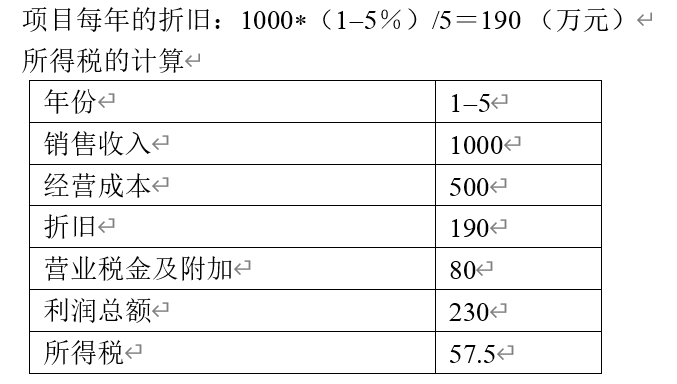
\includegraphics[width=0.8\linewidth]{image/税金-企业所得税.png}
\end{figure}

\subsubsection{总结}
总结:各种税金的计入方向、对现金流的影响(上机时会用到)

(1)增值税当不含税价格时,不考虑,含税价格时单列;

(2)消费税、城市维护建设税、资源税、教育费附加等计入营业税金及附加为现金流出,同时在计算利润时从收入中扣除;

(3)所得税从利润总额中征收,计入所得税,为一项现金流出。

\noindent 考察例题:

\noindent \textbf{例1:}(多选)下列说法错误的是\\
A.机会成本任何时候都不影响现金流量\\
B.经营成本是现金流出\\
C.总成本费用是现金流出\\
D.沉没成本影响项目未来的现金流\\
E.流动资金投资是现金流出\\
\textbf{例2:}(判断题)经营成本=总成本费用-折旧费-摊销费+借款利息支出。\\
\textbf{例3:}(判断题)增值税是价外税。\\
\textbf{答案:ACD;错误;正确。}

\subsection{利润(要求理解并掌握)}
销售利润=销售收入-产品销售成本-产品营业(销售)税金及附加-销售费用-管理费用-财务费用

即销售利润=销售收入-总成本费用-产品营业(销售)税金及附加

税后利润(净利润)=销售利润-所得税

\noindent \textbf{例1:}某项目固定资产原值1000万元,预计固定资产净残值率为5\%,生产期第一年开始按照直线折旧法折旧,折旧年限10年,预计年销售收入1000万元,年经营成本600万元,年营业税金及附加100万元。生产期内每年的利润总额为多少?\\
答:
\begin{figure}[H]
    \centering
    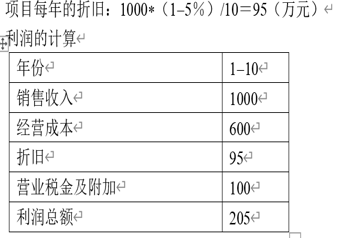
\includegraphics[width=0.8\linewidth]{image/利润总额.png}
\end{figure}
\begin{figure}[H]
    \centering
    \caption{销售收入、成本、税金和利润关系图}
    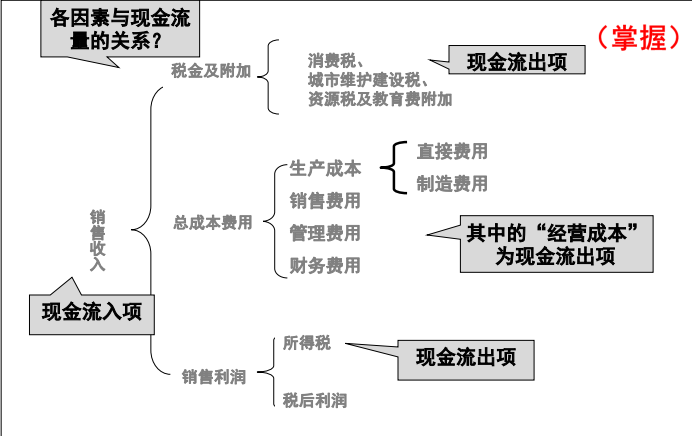
\includegraphics[width=0.8\linewidth]{image/销售收入、成本、税金和利润关系图.png}
\end{figure}
\noindent \textbf{例2:}(多选)以下为现金流出项的为:\\
A.所得税;B.经营成本;C.销售收入;D.城市维护建设税\\
\textbf{答案:}ABD。

\section{按期间构成的项目现金流量}

现金流量的构成与计算:初始现金流量(Initial Cash Flow)、营业现金流量(Operating Cash Flows)、终结现金流量(Terminal Cash Flow)。

\begin{figure}[H]
    \centering
    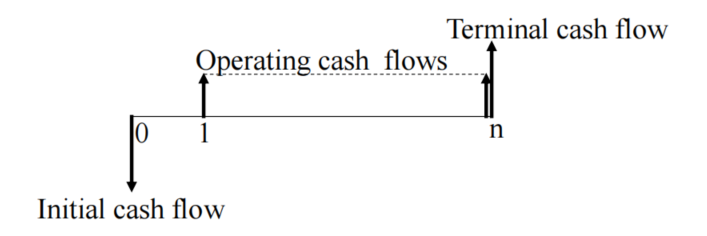
\includegraphics[width=0.8\linewidth]{image/现金流量的构成.png}
    \caption{现金流量的构成}
\end{figure}

\subsection{初始现金流量}
\subsubsection{(1)固定资产投资}
固定资产的购置成本或建造费用,以及运输费、安装费等。
\subsubsection{(2)流动资金投资}
即流动资金,包括对原材料、在产品、产成品和现金等方面的投资。
\subsubsection{(3)其他投资费用}
如职工培训费、谈判费、注册费等开办费。
\subsubsection{(4)原有固定资产变价的税后净收入(设备更新决策)}


\subsection{营业现金流量}
\subsubsection{(1)营业收入}
\subsubsection{(2)税金及附加}
\subsubsection{(3)经营成本}
\noindent 经营成本=总成本费用-折旧和摊销-利息
\subsubsection{(4)所得税}
\subsubsection{(5)计算}
\noindent 营业净现金流量\\
=营业收入-经营成本-税金及附加-所得税\\
=营业收入-(总成本费用-折旧/摊销-利息)-税金及附加-所得税\\
=营业收入-总成本费用-税金及附加-所得税+折旧/摊销+利息\\
=销售利润-所得税+折旧、摊销+利息\\
=税后利润+折旧、摊销+利息

\subsection{终结现金流量}
\subsubsection{(1)固定资产预计净残值}
\subsubsection{(2)流动资金投资回收}

\section{现金流量图}
\subsection{含义}
现金流量图是表示项目系统在整个寿命周期内各时间点的现金流入和现金流出状况的一种图示。

\subsection{绘法}
(1)以横轴为时间坐标,时间间隔相等,时间轴上的点称为时点,时点表示该期的期末,同时也是下一期的期初,零时点即为第一期开始之时点。

(2)以纵轴为现金流量坐标,单位可取元、或万元。

(3)与横轴相连的垂直线,箭头向上表示现金流入,向下表示现金流出,长短与现金流量绝对值的大小成比例,箭头处一般应标明金额。

$\downarrow$ 表示现金流出:某一个时间点的流出系统的固定资产投资;流动资金投资;经营成本;销售税金及附加;所得税。

$\uparrow$ 表示现金流入:某一个时间点的流入系统的资金销售收入;固定资产残值回收;流动资金回收

同一个时间点的现金流入与现金流出的差额叫净现金流量。

系统的现金流入、现金流出和净现金流量统称为现金流量。

一般情况,时间单位为年,假设投资发生在年初,销售收入、经营成本及残值回收等均发生在年末。
$$
\mbox{固定资产净值 = 固定资产原值 - 累计折旧}
$$

期末残值:项目寿命期结束时固定资产的残余价值。

\subsection{现金流量图的进一步说明}
时点:时间坐标的原点通常取在建设期开始的时点,也可取在投产期开始点,而分析计算的起始时间一般都规定在时间坐标的原点。

为了统一绘制方法和便于比较,通常规定投资发生在各时期的期初,而销售收入、经营成本、利润、税金等,则发生在各个时期的期末,回收固定资产净残值与回收流动资金在项目经济寿命周期终了时发生。

第t时点,既表示是第t期末,也表示是第t+1期初。

\textbf{例1:}某工程投资为120万元,一年投产。年销售收入为100万元,年折旧费为20万元,计算期n为6年,固定资产残值为零,年经营成本为50万元,所得税税率为25\%。试求年净现金流量并画出现金流量图。

\textbf{解:}令A为该项目投产后年净现金流量,则:

初始现金流量=-120

营业年现金流量=税后利润+折旧

税后利润=年收入-年总成本费用-年所得税$=(100-50-20)-(100-50-20) \times 25\%=22.5$万元

营业年现金流量$=22.5+20=42.5$万元

现金流量图:
\begin{figure}[H]
    \centering
    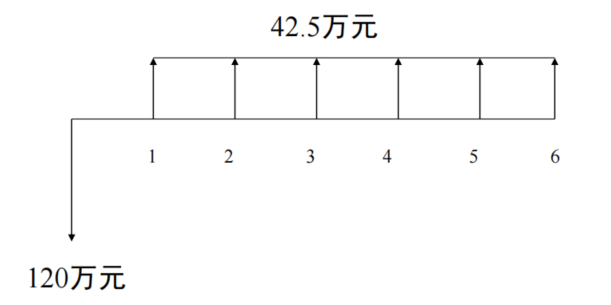
\includegraphics[width=0.75\linewidth]{image/现金流量图-例题.png}
\end{figure}

\textbf{例2:}有一投资项目,固定资产投资50万元,流动资金投资20万元,均于第1年年初投入。项目当年建成投产,产品销售第1年为50万元,第2-7年为80万元;经营成本第1年为30万元,第2-7年为45万元;第1-7年折旧费每年为6万元,第7年末处置固定资产可得收入8万元,所得税税率为25\%。编制该项目的现金流量表。

\begin{figure}[H]
    \centering
    \caption{项目生产期各年的(调整)所得税:}
    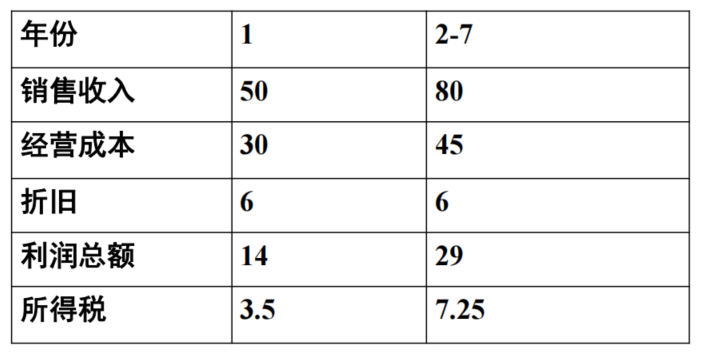
\includegraphics[width=0.75\linewidth]{image/项目生产期各年的(调整)所得税.png}
\end{figure}

\begin{figure}[H]
    \centering
    \caption{项目投资现金流量表}
    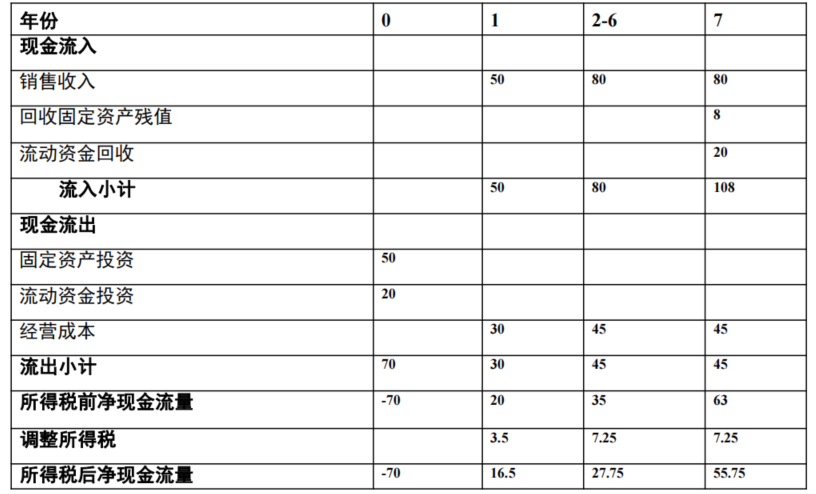
\includegraphics[width=\linewidth]{image/项目投资现金流量表.png}
\end{figure}

\section{现金流量表}
\begin{figure}[H]
    \centering
    \caption{现金流量表}
    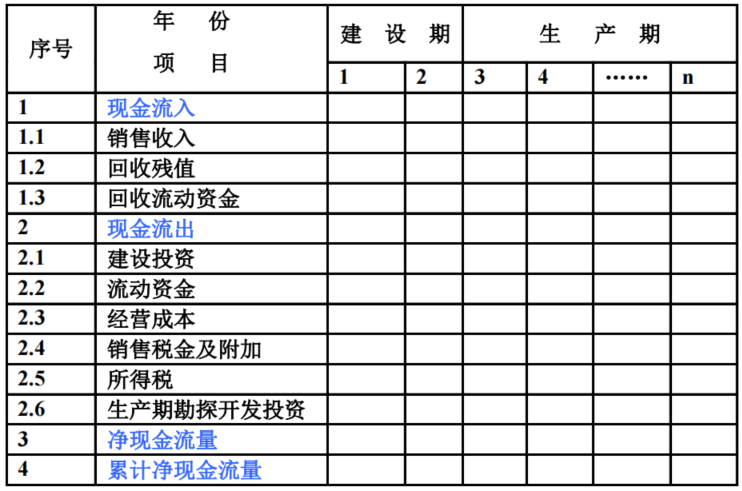
\includegraphics[width=1\linewidth]{image/现金流量表.png}
\end{figure}

\section{分析现金流量应注意的问题(需要理解掌握)}
\noindent \textbf{注意折旧对所得税的影响}

折旧不是现金流出,但不同的折旧方法将影响企业税前利润的计算,从而影响企业的所得税支出,影响现金流量。

\noindent \textbf{沉没成本不是现金流:}以往发生的与当前经营决策无关的成本。
\noindent \textbf{考虑机会成本的影响}

当一种资源用于多种用途时所放弃的其他投资机会中最佳的投资机会。

\noindent \textbf{注意流动资金的投入和收回}

\noindent \textbf{注意财务成本}

例:(多选)下列费用中()不是现金流量\\
A.原材料\\
B.折旧\\
C.沉没成本\\
D.管理费用\\
答案:BC。

\section{总结}
\noindent \textbf{本节重点}\\
1、总投资的两大构成\\
2、固定资产的各种计价\\
3、固定资产折旧方法(直线法)\\
4、对折旧、摊销的理解\\
5、会计和技术经济中成本费用的区别\\
6、技术经济中的四种成本\\
7、各种税对现金流量的影响\\
8、营业收入、成本、税金和利润关系图

\textbf{思考题1:}承德某饮品企业L和江苏某IT企业J均为上市公司,2000年的年报数据表明这两家公司有良好的业绩表现,但L企业采用直线折旧法折旧,而J企业采用加速折旧法,分析这两家企业的发展策略。

\textbf{思考题2:}某公司固定资产投资为5万元,该资产有效期为3年,不考虑折旧前提下,该公司所产生的营业利润为:第一年2万元,第二年3万元,第三年2.5万元。该项目的流动资金为1.5万元。该项目的现金流是多少?

\textbf{思考题3:}某企业购入一项原价24300元的固定资产,估计残值为300元,使用寿命期为4年,试用直线折旧和双倍余额折旧方法分别计算每年的折旧额,累计折旧额和账面资产净值。
\chapter{资金的等值计算}
\section{资金的时间价值(注重理解)}
资金的价值既体现在额度上,同时也体现在发生的时间上。不同时间发生的等额资金在价值上的差别,就称为资金的\textbf{时间价值}。

\textbf{引例1:}C公司年初从Y银行借入1000万元,并约定借期为N年,贷款年利率为6\% ;

(1)从C公司角度看,借用他人的资源,是要付出代价的,即利息,并且时间越长,付出的代价(成本、费用)越多。(与I和N都有关系)。

(2)从Y银行角度看,经营借贷业务的主要目的是通过利息赢利。并且时间越长,增值(赢利)越多。

\textbf{引例2:}现在的500万元,与将来(5年后)的500万元,在价值上不等。那么,现在的500万元,与将来(5年后)的多少万元,在价值上相等?(年利率12\%)。

资金随着时间的推移,会产生价值的变化——增值。

时间越长,资金的增值越多。表现为:利息多了、利润多了等等。

计量增值的方法可以用总利息或利润的多少来计量,也可以用单位时间的利息或利润的多少来计量,即用利率来计量。反时间方向来认识这一现象,就是“将来时间上的一笔数额的资金,在现在看来是不值那么多的”。

\textbf{资金具有时间价值的内涵:}

资金在生产与交换过程中由于有劳动者的劳动使之产生了增值。资金的时间价值是对放弃现时消费的必要补偿。

\subsection{影响资金使用的因素}

\begin{itemize}
    \item 投资收益率
    \item 风险
    \item 通货膨胀
\end{itemize}

\subsection{概念}
不同时间发生的等额资金在价值上的差别称为资金的时间价值。也即资金在生产和流通过程中随着时间推移而产生的增值。

对资金使用者来讲,是使用资金的成本。

如:某项目投资100万元,建成投产后,每年可得利润20万元,即为100万元在特定生产经营活动中所产生的时间价值。

\subsection{涵义}
(1)资金随着时间的推移,其价值会增加。

(2)从消费者角度讲,是对放弃现期消费的补偿。

\subsection{资金时间价值表现形式}
一是资金投入生产或流通领域产生的增值称为利润(Profit)或收益(Income);

二是把资金存入银行或向银行借贷所得到或付出的增值额称为利息(Interest)。

\subsection{资金时间价值衡量尺度}
(1)绝对尺度:体现资金时间价值绝对量的多少。利息、利润或收益;

(2)相对尺度:反映资金时间价值相对量的大小。利息率、利润率或收益率。

\subsection{资金时间价值的意义}
项目的经济评价中,必须增强资金的时间观念,用动态的观点看待资金的使用,考虑资金的时间价值,采用动态分析方法将不同的费用或效益折算成同一时点来进行比较。

\subsection{资金等值的概念}

资金等值是指在不同时点绝对值不等而价值相等的资金。

在一个或几个项目中,投资或收益往往发生在不同的时间,于是就必须按照一定的利率将这些投资或收益折算到某一个相同的时点,这一过程就是等值计算。

\section{利息和利率}
\subsection{利息$I_n$}
贷款人向借款人让渡资金使用权而得到的一种报酬,也是借款人占用资金所付的代价。

某人存入银行一笔资金,存期\textbf{5年}(\textbf{计息期}),\textbf{每年}(\textbf{计息周期(每次计算利息的时间单位)})计息一次,整个存储期间共计息\textbf{5次}(\textbf{n:计息周期次数})。

\subsection{利息的表示方式}
\subsubsection{(1)绝对数表示:}
$$I_n = F_n - P$$
$F_n$:经过$n$个计息周期后的本利和。
\subsubsection{(2)相对数表示:}
指单位本金经过一个计息周期的利息数额。
$$i = \frac{I_1}{P} \times 100\%$$

\subsection{利率i}

一定时期内(一年、半年、月、季度,即一个计息周期)利息总额与本金(借贷金额)的比率。

$$\mbox{利率} = \frac{\mbox{期利息}(I_1)}{\mbox{本金}(P)} \times 100\%$$

利率是单位本金经过一个计息周期后的增殖额。(年利率、半年利率、月利率,……)

\subsection{利息计算方法}
\subsubsection{(1)单利法}

仅对本金计息,利息不再生利息。
$$I_n= p \cdot n\cdot i$$
$$F_n=P \cdot (1+i \cdot n)$$

P为本金,n为计息期数(通常为年),i代表利率,I代表所付或所收的总利息,F代表本利和。

\begin{figure}[H]
    \centering
    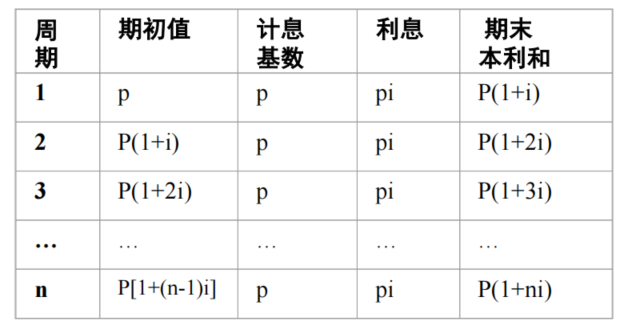
\includegraphics[width=0.9\linewidth]{image/单利法本利和公式推导.png}
    \caption{单利法本利和公式推导}
\end{figure}

\subsubsection{(2)复利法}

核心:以本金与累计利息之和为计息基数,即“利上加利”、“利滚利”、“驴打滚”。

技术经济分析中时间价值一般采用复利法,充分反映资金的时间价值。

\begin{figure}[H]
    \centering
    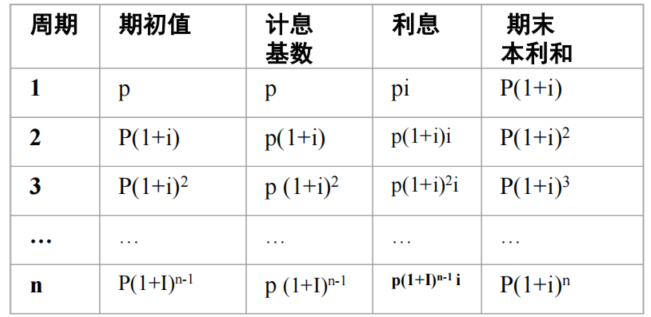
\includegraphics[width=0.9\linewidth]{image/复利法本利和公式推导.png}
    \caption{复利法本利和公式推导}
\end{figure}

$$F_n=P \cdot (1+i)^n$$

\begin{itemize}
    \item $P$:原始本金;
    \item $i$:一个计息周期利率;
    \item $n$:计息期内计息周期次数。
\end{itemize}

\subsubsection{(3)差异分析}
单利计息:对资金时间价值的考虑不完整,利息没转入记息基数;

复利计息:充分反映资金的时间价值。


\subsection{名义利率和实际利率}
\subsubsection{(1)名义利率}
在技术经济分析中,复利计算通常以年为计息周期。但在实际经济活动中,计息周期有年、半年、季、月等多种,这样出现了不同计息周期的利率换算问题。

如:按月计算利息,且其月利率为1\%,通常称为“年利率12\%,每月计息一次”。这个年利率12\%称为“\textbf{名义利率}”。

名义利率的计算:
$$\mbox{名义利率}(r) = \mbox{每一计息周期的利率} \times \mbox{一年中的计息周期的次数}(m)$$
$$r/m = \mbox{每一计息周期利率}$$

\subsubsection{(2)实际利率}
\textbf{实际利率:}当一年内多次复利计息时,按照一年内获得的利息与年初本金之比计算出的年利率为实际年利率。

实际利率的计算:
$$\mbox{实际利率}(i)=\mbox{一年内按复利计息的利息总额}/\mbox{年初本金}$$\\
举例:
本金1000元,每月复利计息一次,月利率1\%,一年后的本利和为:
$$F = 1000 \times (1+1\%)^{12}= 1126.8 \mbox{(元)}$$
实际利率为:
$$\frac{1126.8-1000}{1000} \times 100\%=12.68\%$$

\subsubsection{(3)名义利率和实际利率公式推导(我认为不需要掌握,但是看两眼)}
复利计息,一年后本利和为:
$$F=P(1+r/m)^m$$

一年内的利息额为:
$$I=F-P=P \times (1+r/m)^m-P=P \times [(1+r/m)^m-1]$$

实际利率为:
$$i=(F-P)/P=\frac{P \times (1+r/m)^m-p}{p}=(1+r/m)^m-1$$

若计息周期为一年,$m = 1$,则$i = r$,即实际利率=名义利率。

若连续计息, $m \to \infty$,则:
$$i = \lim_{m \to \infty}(1+\frac{r}{m})^m-1=e^r-1$$

若名义年利率为12\%,以下各种情况下,实际年利率等于多少?

\textcircled{1}按年计息,m=1
$$i = (1+ r/m)^m-1=(1+0.12/1)^1-1=12\%$$

\textcircled{2}按半年计息,m=2
$$i = (1+ r/m)^m-1=(1+0.12/2)^2-1=12.36\%$$

\textcircled{3}按季度计息,m=4
$$i = (1+ r/m)^m-1=(1+0.12/4)^4-1=12.55\%$$

\textcircled{4}按月计息,m=12
$$i = (1+ r/m)^m-1=(1+0.12/12)^{12}-1=12.68\%$$

\textcircled{5}按连续计息,m=$\infty$
$$i=e^r-1=e^{0.12}-1=12.75\%$$
\textbf{例1:}某人将1000元存入银行,定期3年,年利率12\%,3年期满,按复利计算,期满后他可以从银行得到[填空1]元。\\
\textbf{答案:}\\
实际利率:$i=(1+\frac{12\%}{12})^{12}-1=1.01^{12}-1=12.68\%$\\
应归还本利和:$20 \times (1+12.68\%)^3=20 \times 1.4308=28.62$(万元)\\
\textbf{例2:}下列说法正确的是\\
A. 名义年利率条件下,一年的利息额是按单利计算
\\
B. 实际年利率条件下,一年的利息额是按单利计算
\\
C. 实际年利率条件下,一年的利息额是按复利计算
\\
D. 名义年利率条件下,一年的利息额是按复利计算\\
\textbf{答案:}AC\\
\textbf{例3:}(判断题)若一年中复利计息的次数大于1,则年实际利率小于年名义利率。\\
\textbf{答案:}错误\\
差异原因分析:
$$\mbox{年利率}i=\frac{\mbox{一年的利息额}}{\mbox{年初本金}} \times 100\%$$
名义年利率:一年的利息额是按单利计算的;\\
实际年利率:一年的利息额是按复利计算的;\\
当一年中多次计息时(即$m>1$时),两者产生差异。


\section{资金的等值计算}

\subsection{基本概念}

资金的时间价值:在不同的时间付出或得到同样数额的资金在价值上是不等的,即资金的价值会随着时间发生变化。

评价技术的经济效果,不仅要考虑现金流入、流出的数额,还要考虑每笔现金流量发生的时间。

不同时间发生的等额资金在价值上的差别称为资金的时间价值。也即资金在生产和流通过程中随着时间推移而产生的增值。对资金使用者来讲,是使用资金的成本。

某项目投资100万元,建成投产后,每年可得利润20万元,即为100万元在特定生产经营活动中所产生的时间价值。

\subsubsection{决定资金等值的因素}
\begin{itemize}
    \item 资金数额
    \item 资金发生的时刻
    \item 利率:关键因素
\end{itemize}

资金随着时间的推移,其价值会增加。从消费者角度讲,是对放弃现期消费的补偿。

\subsubsection{资金的时间价值引发的问题}

\begin{figure}[H]
    \centering
    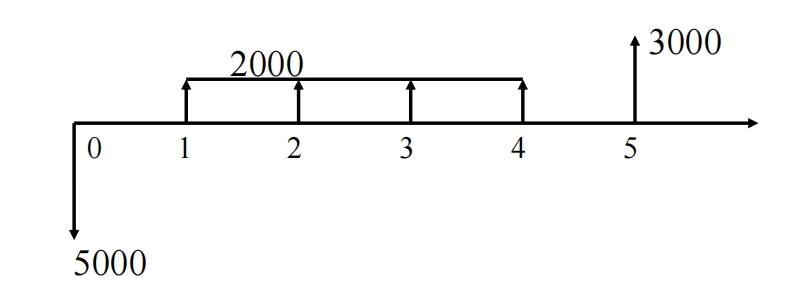
\includegraphics[width=0.8\textwidth]{image/资金时间价值引发的问题.png}
    \caption{资金时间价值引发的问题}
    \label{fig:3}
\end{figure}

不能直接比较不同时间点的资金的价值大小;

需要利用等值换算,将不同时点的资金换算到同一时点进行比较。

\subsubsection{资金时间价值表现形式}
\begin{itemize}
    \item 资金投入生产或流通领域产生的增值称为利润(Profit)或收益(Income)。
    \item 把资金存入银行或向银行借贷所得到或付出的增值额称为利息(Interest)。
\end{itemize}

\subsubsection{资金时间价值衡量尺度}
(1)绝对尺度:体现资金时间价值绝对量的多少。利息、利润或收益;

(2)相对尺度:反映资金时间价值相对量的大小。利息率、利润率或收益率。

\subsection{资金等值}
\subsubsection{概念}
在考虑资金时间价值的情况下,在不同的时间绝对值数额不等的若干资金,如果具有相同的价值,则为等值的资金。

例如,年初的100元和年底的110元,在单利10\%的情况下是等值的。

\subsubsection{资金等值概念的意义}
利用等值概念,通过等值计算,可以知道某一时点上的资金金额在其他时点上的价值。可以把不同时点发生的资金金额换算到同一时点进行价值比较。
\subsubsection{相关概念}
等值资金:在利率一定的条件下,我们把不同时间(时期、时点)上绝对数额不等,而经济价值相等的若干资金,称为等值资金。

资金等值计算:利用资金等值原理,我们可以把某一时间点上的资金值,按照所给定的利率换算为与之等值的另一时间点的资金值,这一换算过程称为资金的等值计算。

折现(贴现Discount):把将来某一时间点上的资金值换算成现在时间点上的等值资金值。

折现率($i$,Discount Rate):进行资金等值计算中使用的反映资金时间价值的参数叫折现率。(如利率、收益率)

现值($P$,Present Value):“现值”并非专指一笔资金“现在”的价值,它是一个相对的概念。一般地说,将$t+k$个时点上发生的资金折现到第$t$个时点,所得的等值金额就是$t+k$个时点上的资金金额的现值。

终值($F$,Future Value):与现值等价的将来某时点的资金值称为“终值”。

等年值($A$,年金,Annual Value):分期等额收支的资金值。\\
\textbf{例题:}(判断)折现是指将来时点的资金金额换算成期初时点的资金金额这一过程。\\
\textbf{答案:}错误。

\section{资金等值计算公式(重点掌握)}
按照现金流的不同,等值公式可以分为:

一次收付类型:两个

等额分付类型:四个(另引申四个)

等差序列类型(自学,了解)

等比序列类型(自学,了解)

\subsection{一次收付型}
是指所分析系统的现金流量,无论是流入还是流出,均在一个时间点上一次发生。包括:

一次收付终值(未来值)公式

一次收付现值公式

\subsubsection{一次收付终值公式($P \to F$)}

\begin{figure}[H]
    \centering
    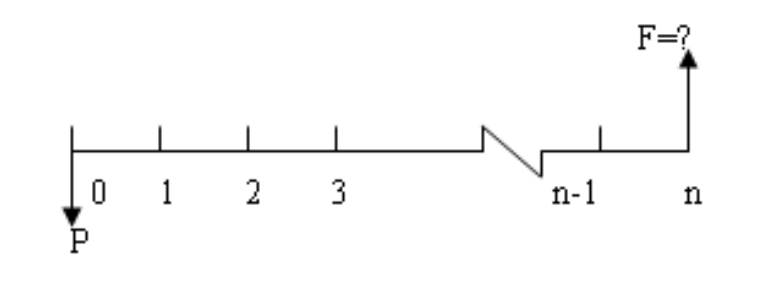
\includegraphics[width=0.8\textwidth]{image/一次收付终值现金流量图.png}
    \caption{一次收付终值现金流量图}
    \label{fig:3}
\end{figure}

已知$P$,求$F$,即求$P$在$n$年后的等值资金$F$

复利终值计算公式:\\
(与复利计息本利和计算公式相同)
$$F=P \cdot (1+i)^n$$

或

$$F=P \cdot (F/P,i,n)$$



\textbf{整付终值计算公式}

已知期初投资为$P$,利率为$i$,求第n年末收回本利$F$。
$$F=P(1+i)^n$$

$(1+i)^n$称为整付终值系数,记为$(F/P,i,n)$。

$(F/P,i,n)$中,$F$为欲求因素,其余为已知因素。复利终值系数可查表,如图\ref{fig:5}:

\begin{figure}[H]
    \centering
    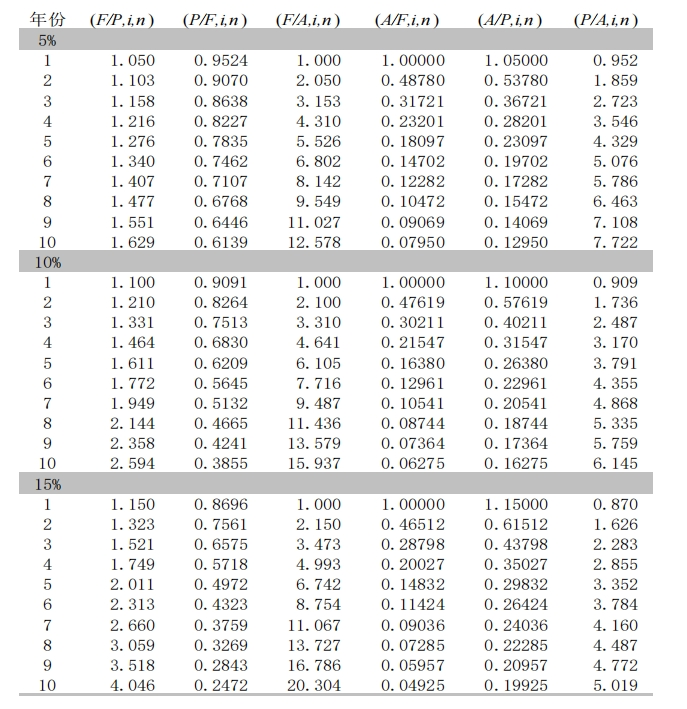
\includegraphics[width=\textwidth]{image/复利终值系数表.png}
    \caption{复利终值系数表}
    \label{fig:5}
\end{figure}

\subsubsection{一次收付现值公式($F \to P$)}
即在已知利率$i$的条件下,要想在$n$期期末得到资金$F$,期初应一次投入多少资金?其现金流量图如图\ref{fig:6}所示。

\begin{figure}[H]
    \centering
    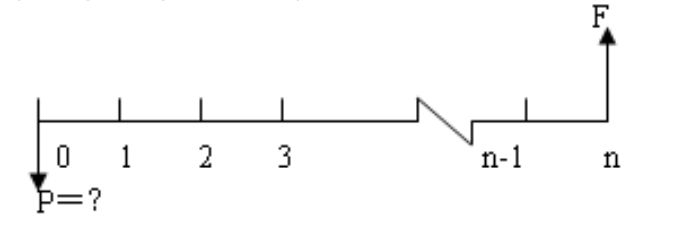
\includegraphics[width=0.8\textwidth]{image/一次收付现值现金流量图.png}
    \caption{一次收付现值现金流量图}
    \label{fig:6}
\end{figure}

\textbf{复利现值计算公式}
$$P=\frac{F}{(1+i)^n}=F \cdot (1+i)^{-n}$$(一次支付终值公式的逆运算)\\
或
$$P=F \cdot (P/F,i,n)$$(复利现值系数与复利终值系数互为倒数)\\
\textbf{例1:}给你一次选择机会,你可以现在获得1000元,也可以在5年以后的今天获得1300元,在年利率为8\%的情况下,你将做何种选择?\\
\textbf{答案:}$P=F/(1+0.08)^5=1300/(1+0.08)^5=884.76$\\
由于在年利率为8\%时, 5年后的1300元等值于现在的884.76元,小于同一时点的1000元,故应该选择现在获得1000元。\\
\textbf{例2:}某人把1000元存入银行,设年利率为6\%,复利计息,5年后全部提出,共可得多少元?

$F=P(1+i)^n=1000 \times (F/P,6\%,5)=1000 \times 1.338=1338$(元)\\
\textbf{例3:}某环保制造企业计划建造一条生产线,预计5年后需要资金1000万元,设年利率为10\%,复利计息,问现需要存入银行多少资金?

$P=F(1+i)^{-n}=1000 \times (P/F,10\%,5)=1000 \times 0.6209=620.9$(万元)

\subsection{等额分付系列公式}

含义:
等额分付是多次支付形式的一种,多次支付指现金流入和流出在多个时点上发生,而不是集中在某个时点上。当现金流序列是连续的,且数额相等,则称为等额系列现金流。
\begin{itemize}
    \item 等额分付年金终值公式
    \item 等额分付偿债基金公式
    \item 等额分付年金现值公式
    \item 等额分付资本回收公式
\end{itemize}

\subsubsection{等额收付年金终值公式($A \to F$)}

若每期期末支付同等数额的资金$A$,在利率为$i$的情况下,$n$期后的未来值应该是多少?其现金流量图如图\ref{fig:7}所示。

\begin{figure}[H]
    \centering
    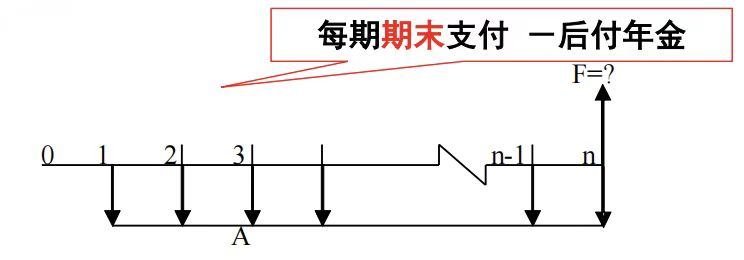
\includegraphics[width=0.8\textwidth]{image/等额收付终值现金流量图.jpg}
    \caption{等额收付终值现金流量图}
    \label{fig:7}
\end{figure}

\noindent \textbf{年金终值公式:}
$$F=A(1+i)^{n-1}+A(1+i)^{n-2}+\mbox{…}+A(1+i)+A=A \sum_{i=1}^{n} (1+i)^{n-1}=A[\frac{(1+i)^n-1}{i}]$$(利用等比级数求和公式)\\
或
$$F = A(F / A, i, n)$$(年金终值系数)\\
\textbf{例题:}某人从现在开始的三年内每年年末存入银行1000元,存款利率为10\%,复利计息,计算第三年年末该人银行账户的余额。\\
\textbf{答案:}$F=A \cdot (F/A,10\%,3)=1000 \times 3.310 = 3310$(元)\\
\textbf{引申:}如果上例改为“三年内每年年初存入银行1000元”,其他条件不变,则第三年年末该人银行账户的余额为多少?\\
\textbf{答案:}$F_d=A(F/A,10\%,3) \times (1+i)=1000 \times 3.310 \times (1+10\%)=3641$(元)

\noindent \textbf{先付年金}

$$F_d= A \cdot ( F / A , i , n ) \cdot (1 + i)$$

\begin{figure}[H]
    \centering
    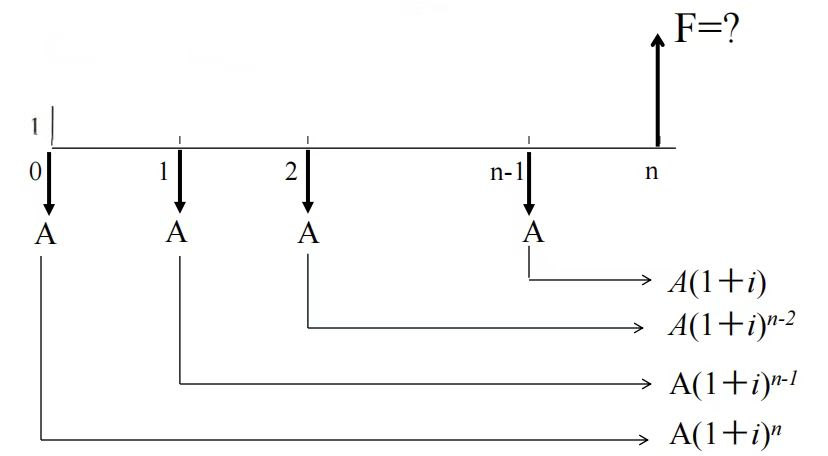
\includegraphics[width=0.8\textwidth]{image/先付年金图示.jpg}
    \caption{先付年金图示}
    \label{fig:8}
\end{figure}

\subsubsection{等额分付偿债基金公式($F \to A$)}
等额收付偿债基金公式是等额分付终值公式的逆运算。即已知终值F,求与之等值的等额年金A。\\
\textbf{偿债基金公式:}
$$A=F[\frac{i}{(1+i)^n-1}]$$
\textbf{偿债基金系数:}
$$A = F ( A / F , i , n )$$
\textbf{例题:}某人5年后需要10万元,他准备从现在起每年年末向银行存入一笔等额金额,已知存款年利率为5\%,复利计息,问每年的等额存款是多少?\\
\textbf{答案:}$A=100000(A/F,5\%,5)=100000 \times 0.18097)=18097$(元)\\
\textbf{引申:}如果上例改为每年年初向银行存入一笔等额金额,则每年的等额存款是多少?(提示:先付年金终值公式的逆运算)\\
\textbf{答案:}$A=100000(A/F,5\%,5)/(1 + 5\%)= (100000 \times 0.18097)/1.05= 17235$(元)

\subsubsection{等额分付年金现值公式$(A \to P)$}
若在每年年末等额分付资金$A$,在利率为$i$的条件下与之经济等值的现值为多少?其现金流量图\ref{fig:9}如图所示。

\begin{figure}[H]
    \centering
    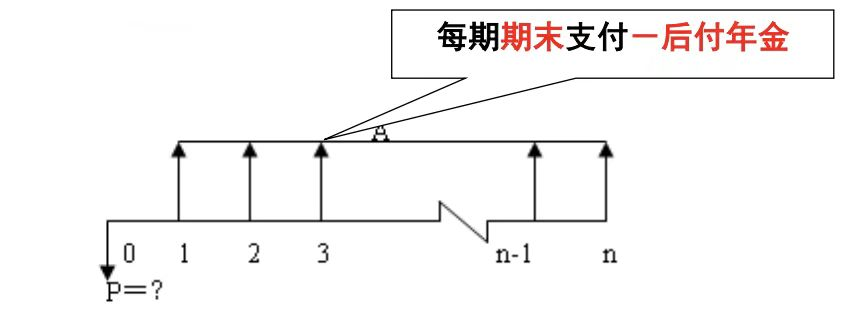
\includegraphics[width=0.8\textwidth]{image/等额收付现值现金流量图.jpg}
    \caption{等额收付现值现金流量图}
    \label{fig:9}
\end{figure}

\noindent \textbf{年金现值公式:}
$$P=A[\frac{(1+i)^n-1}{i(1+i)^n}]$$

\noindent \textbf{年金现值系数:}
$$P=A(P/A,i,n)$$

\noindent \textbf{例题:}某人为了在以后3年内每年年末可以从银行提取1000元,假设存款年利率为10\%,复利计息,问该人现在应该存入多少钱?\\
\textbf{答案:}$P=A(P/A,10\%,3)=1000 \times 2.487=2487$(元)\\
\textbf{引申:}上例中,如果改为“为了在以后3年内每年年初可以从提取1000元”,其他条件不变,则该人现在应该存入多少钱?\\
\textbf{答案:}$P_d=A \cdot (P/A,10\%,3) \cdot (1+i) =1000 \times 2.487 \times (1+10\%)=2735.7$(元)

\noindent \textbf{先付年金现值公式}
$$P_d=A[\frac{(1+i)^n-1}{i(1+i)^n}](1+i)$$
$$P_d=A(P/A,i,n)(1+i)$$

\noindent \textbf{特例——永续年金现值公式}
$$P=\frac{A}{1+i}+\frac{A}{(1+i)^2}+...\frac{A}{(1+i)^n}+...=A\lim_{n \to \infty}[\frac{(1+i)^n-1}{i(1+i)^n}]=\frac{A}{i}$$

\subsubsection{资本回收公式($P \to A$)}
资本回收公式是年金现值公式的逆运算,即已知现值$P$,求与之等值的年金$A$。

$$A=P[\frac{i(1+i)^n}{(1+i)^n-1}]$$

\noindent \textbf{资本回收系数:}
$$A=P(A/P,i,n)$$
\textbf{例题:}某人以分期付款的方式买下一套价值20万元的房子,年利率为8\%,付款期限为15年,每年付款额相等,问此人每年年末需要付多少钱?\\
\textbf{答案:}$A=200000(A/P,8\%,15)=200000 \times 0.11683=23367$(元)\\
\textbf{引申:}在上例中,如问此人每年年初需要付多少钱?(提示:先付年金现值公式的逆运算)\\
\textbf{答案:}$A=200000(A/P,8\%,15)/(1+i)=(200000 \times 0.11683)/(1+8\%)=21636$(元)

\section{本章思考题(必做)}
\noindent \textbf{思考题1:}某人连续10年每年年初存入银行1000元,名义利率10\%,半年复利计息一次,计算10年末此人存款的本利和是多少?

\noindent \textbf{思考题2:}2、假定第一年年初你存入银行10万元,年利率5\%,从第4年年末开始连续6年每年年末从银行取出相等的金额,使得存款账户余额为0。问每年取出的金额是多少?

\noindent \textbf{思考题3:}在你出生时,你的父母决定在你的每一个生日为你存款1000元,直到18岁。但是你的父母在你7岁和11岁时没有存款,假设年利率为5\%,当你18岁时,银行账户的余额是多少?

\noindent \textbf{思考题4:}某人与保险公司订立了一份养老保险合同。合同规定此人现在支付保险公司100,000元,在此后的15年中保险公司每年末付给他10,000元,问保险公司提供的年利率是多少?(给出利率区间即可)

\noindent \textbf{思考题5:}某人希望拥有100,000元的存款,为了实现这一目标,他计划从现在开始每年年初存入5,000元,年利率为8\%,问需要多少年?

\noindent \textbf{思考题6:}若年利率为13\%,连续n期期初年金的现值为46.38元,则连续n期期末年金的现值为多少?
\chapter{基准折现率的确定}
基准折现率(基准收益率)是衡量项目可行性和方案比选的主要依据。它反映投资者对项目占用资金时间价值的判断,是投资者从事投资活动可接受的下临界值。其高低直接影响着经济评价决策指标的计算结果。如从$NPV(i)$的特性看,$i$定的越大,$NPV$越小,表明对项目要求越严,审查越严。

一个例子,你去玩一个游戏,赢了这个游戏给你100块钱,输了就什么都没有,输赢的概率都是50\%。此时给你两种选择:要么玩;要么你不参加游戏,直接给你50块钱。你的选择是?

那么,如果你去玩一个游戏,赢了这个游戏给你200块钱,输了就什么都没有,输赢的概率都是50\%。还是同样的两种选择:要么玩;要么你不参加游戏,直接给你50块钱。你的选择又是什么呢?

因此,我们确定基准折现率时,需考虑的因素如下:
机会成本、风险、资本成本、通胀。

\section{风险与收益}
\subsection{风险的概念}
风险是指投资者未来收益的不确定性。
\subsection{风险投资原则}
\begin{itemize}
    \item 同风险、同收益;
    \item 高风险,高收益;
    \item 低风险,低收益。
\end{itemize}

\subsection{股票、债券的报酬率}
\subsubsection{股票的报酬率}
$$\mbox{报酬率}=\mbox{股利收益率}+\mbox{资本利得收益率}=\frac{\mbox{期末支付的股利}+\mbox{当期市场价值的变动}}{\mbox{期初市场价值}}$$

\subsubsection{债券的报酬率}
通过长期的观察发现,债券的报酬率远低于股票的报酬率,国库券的报酬率很低。如买政府的国库券,几乎没有任何违约风险,此时的收益率可看成无风险报酬率。

\subsubsection{风险溢酬}
风险非常大的股票的报酬率和国库券的报酬率差额是超额报酬率。可以被解释为承担风险的报酬,称为\textbf{风险溢酬}。风险性资产会赚取风险溢酬,即承担风险就会有回报。而且通过对股票、债券等计算其\textbf{方差和标准差},发现报酬率越高,其标准差就越大,也就是在某一给定的年度,股票价值出现特别大的变动的机会就很大,说明收益率越高,风险越大。
$$\mbox{风险溢酬}=\mbox{期望报酬率}-\mbox{无风险报酬率}$$

\subsection{投资组合的报酬率及风险}

\begin{figure}[H]
    \centering
    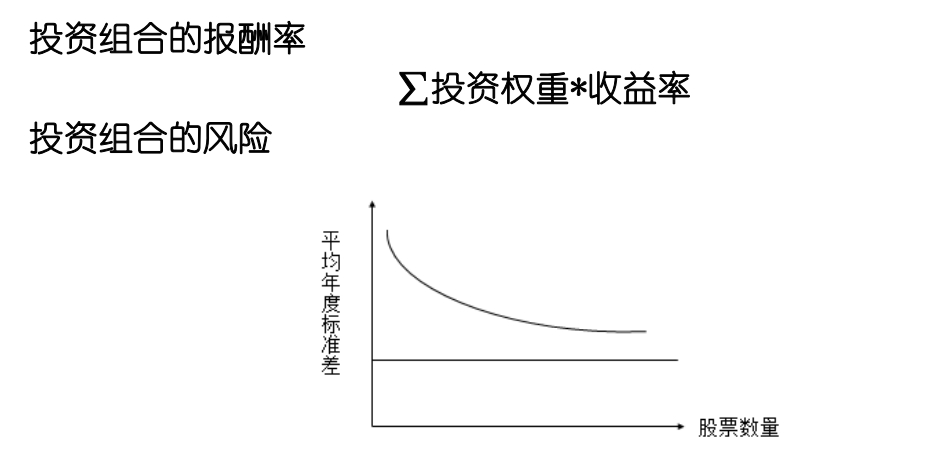
\includegraphics[width=0.9\textwidth]{image/投资组合的报酬率及风险.png}
    \caption{投资组合的报酬率及风险}
    \label{fig:10}
\end{figure}

\subsection{系统风险和非系统风险}
\textbf{系统风险(市场风险)}:对整个市场有影响,比如总体经济状况的不确定性,利率、经济衰退、战争等,属不可分散风险。

\textbf{非系统风险(特有风险或者具体资产风险)}:影响某个单项资产或一小组资产,是个别公司或者资产特有的,属可分散风险。
$$\mbox{整体风险}=\mbox{系统风险}+\mbox{非系统风险}$$

通过分散化化解非系统风险几乎没有任何成本,因此承担这种风险没有回报。
承担风险时所得到的回报的大小,仅取决于系统风险。也即一项资产的期望报酬率取决于系统风险。

通常用$\beta$衡量不同投资的系统风险水平。平均资产的$\beta$为1。

\begin{figure}[H]
    \centering
    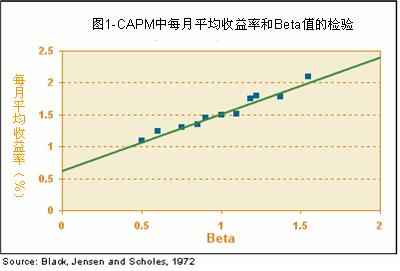
\includegraphics[width=0.8\textwidth]{image/CAPM中每月平均收益率和Beta值的检验.jpg}
    \caption{CAPM中每月平均收益率和Beta值的检验}
    \label{fig:11}
\end{figure}
$$\mbox{期望报酬率}=\mbox{无风险报酬率}+\mbox{市场风险溢酬}$$
$$R_E=R_f+[E(R_M)-R_f]*B_i$$

$R_f$:无风险报酬率;

$[E(R_M)-R_f]$:市场平均风险溢酬;

$B_i$:一项特定资产相对于平均资产而言,所面临的系统风险的大小。

\section{资本成本的确定}
\subsection{企业筹资的类别}
\textbf{权益资金(Equity)}是由企业所有者投入的资金,企业可长期使用,无需偿还。

\textbf{债务资金(Debt)}是由企业债权人投入的资金,企业需按约使用,按期偿还。

资本成本(cost of capital)是指投资者投资于企业的必要预期收益率。因此,资本成本与投资者投资于企业所承担的风险有关。

权益投资者承担相对较高的风险,因此权益资本成本较大。权益投资者承担的风险用贝塔系数来衡量。

债务投资者(债权人)承担相对较低的风险,因此债务成本较低。

\subsection{债务资本成本的计算}
\subsubsection{债券定价公式}
$$P=\sum_{t=1}^{n} \frac{I}{(1+r_D)^t}+\frac{F}{(1+r_D)^n}$$

$I$:各期的利息,等于票面值乘以票面利率。

$F$:债券面值。

$n$:债券到期期限。

$r_D$:债券的到期收益率,或债券资本成本。\\
\textbf{例题:}A公司发行的债券,面值为1000元,票面利率10\%,期限为10年。目前该债券还有8年到期,当前的市场价格为1050元。计算该债券的到期收益率或资本成本。\\
\textbf{答案:}
$$1050=\sum_{t=1}^{8}\frac{100}{(1+r_D)^t}+\frac{1000}{(1+r_D)^8}$$
$$r_D=9\%$$

\subsection{权益资本成本的计算}
利用资本资产定价模型(CAPM)
$$r_E=r_F+\beta \cdot (r_M-r_F)$$
式中:\\
$r_E$:权益必要收益率或权益资本成本;\\
$r_F$:无风险收益率;\\
$r_M$:市场平均收益率;\\
$\beta$:企业权益的风险系数。\\
\textbf{例题:}A公司的$\beta$系数为1.15,无风险收益率为6\%,市场平均收益率为14\%,计算A公司的权益资本成本。\\
\textbf{答案:}$r_E=6\%+1.15(14\%-6\%)=15.2\%$

\subsection{加权平均资本成本(WACC)}
个别资本成本为税后成本;个别资本的权重为市场价值权重。
$$WACC=\frac{D}{D+E} \times r_D(1-T)+\frac{E}{D+E}  \times r_E$$
式中:\\
$WACC$:加权平均资本成本;\\
$D$:债务的市场价值;\\
$E$:权益的市场价值;\\
$D+E$:企业的市场总价值。\\
\textbf{例题:}A公司现有债务4000万元,债务成本为9\%;权益价值6000万元,权益成本为15.2\%;该公司所得税税率为25\%,计算公司的WACC。\\
\textbf{答案:}$WACC=40\% \times 9\% \times (1-25\%) +60\% \times 15.2\%=11.82\%$

\section{投资风险补偿}
要估计一个适当的风险贴水率,也被称为风险补偿系数 (Risk Adjusted Discount Rate)
$$MARR=k+h$$

$K=Max$(借贷资金成本、加权平均资本成本、机会成本);

$h$:投资风险补偿系数。

\begin{table}[H]
\centering
\begin{tabular}{|l|l|}
\hline
\textbf{风险等级}       & \textbf{h(\%)}                \\ \hline
高度风险(新技术、新产品)      & 20\textasciitilde100        \\ \hline
较高风险(生产活动范围外新项目、新工艺) & 10\textasciitilde20         \\ \hline
一般风险(生产活动范围内市场信息不确切) & 5\textasciitilde10          \\ \hline
较小风险(已知市场现有生产外延)   & 1\textasciitilde5           \\ \hline
极小风险(稳定环境下降低生产费用)   & 0\textasciitilde1           \\ \hline
\end{tabular}
\caption{风险等级与风险百分比}
\end{table}

\section{通货膨胀}
若项目的收入和支出是各年的即时价格计算的必须考虑通货膨胀率;若按不变价格计算的,此项可不考虑。

\section{行业财务基准收益率的主要测定方法(了解即可)}
\subsection{资本资产定价模型}
不同行业的风险不同,风险溢价不同。通过测定行业投资收益变动与市场总投资收益变动的关系,分析行业投资风险的大小。在参数与方法中,行业财务基准收益率(权益资本)的测算采用了资本资产定价模型的思路与方法,并依据我国实际情况变通使用。

无风险收益率一般采用政府发行的相应期限的国债利率,2004年是2.5\%。市场平均风险投资收益率2004年是8\%。

\subsection{WACC(加权平均资本成本)}
通过测定WACC ,可以得出行业内全部投资的最低可用折现率,为确定融资前税前行业财务基准收益率提供参考价下限。在综合考虑各行业收益率并进行协调后,确定全行业基准投资收益率取值。

\subsection{典型项目模拟法}
通过选取行业内一定数量有代表性的已进入正常生产运营状态的建设项目,进行调查,搜集其折现率。当然,项目必须有代表性,典型。在一定典型的基础上,测定行业的。

\subsection{德尔菲专家调查法}
充分利用专家熟悉行业特点、行业发展变化规律、项目收益水平和具有丰富经验的优势,由一定数量的专家对项目收益率取值进行判断,经过几轮,逐步集中。形成结论性取值。

在调查过程中,如果在基本没有人为因素干扰的情况下能形成收敛性的结论,则这一结论能对基准收益率的取值提供重要参考。2006年时组织了全国500多位各行业专家进行调查。

\subsection{总结}
在测算中,无论哪种方法,都要在测算分析的基础上进行必要的调整,最终的取值是综合权衡的结果,而不是简单的计算。

国家行政部门统一测定、发布的行业基准财务收益率对于政府投资项目是规定性的,必须采用的,对于社会其他各类项目,是参考性的。项目评价人员可以根据具体情况选用,也可以自主测定。由投资者自己决定。

如石油行业的陆上气田开采项目,融资前财务基准收益率,专家调查结果是13\%,行业测算结果是12\%,协调结果是12\%。

\begin{figure}[H]
    \centering
    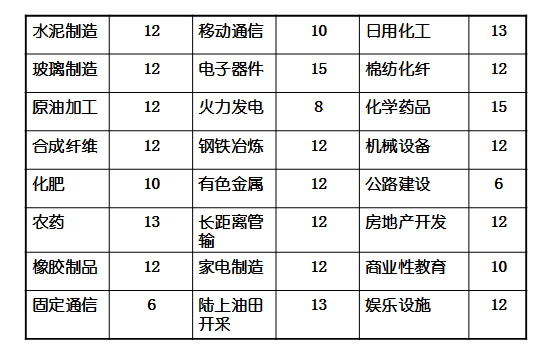
\includegraphics[width=0.9\textwidth]{image/我国行业基准折现率.png}
    \caption{我国行业基准折现率}
    \label{fig:12}
\end{figure}

\chapter{经济效果评价指标}
\noindent{以货币单位计量的价值型指标:}\\
净现值、净年值、费用现值、费用年值等;\\
反映资金利用效率的效率型指标:\\
内部收益率、净现值指数、投资收益率等。

\section{(静态)投资回收期(Payback period)}
\subsection{概念}

从项目投建之日起,用项目各年的净收入(年收入减年支出)将全部投资收回所需的期限。

\begin{equation*}
\sum_{t=0}^{T_p}{(CI-CO)}_t = 0
\end{equation*}

(左边:累积净现金流量)
\begin{itemize}
    \item $T_p$ - 投资回收期
    \item $CI$ - 现金流入量
    \item $CO$ - 现金流出量
    \item $(CI-CO)_t$ - 第t年的净现金流量
\end{itemize}

\subsection{列表法}
如果投产或达产后各年的净收益不等,用列表法(累计净收益法)求得。

\subsection{投资回收期计算}

\begin{equation}
    T_p = (T - 1)+\frac{\sum_{t=0}^{T-1}{(CI-CO)}_t}{{(CI-CO)}_T}
\end{equation}

T为项目各年累积净现金流量首次为正值或零的年份。

案例:
\begin{figure}[h]
    \centering
    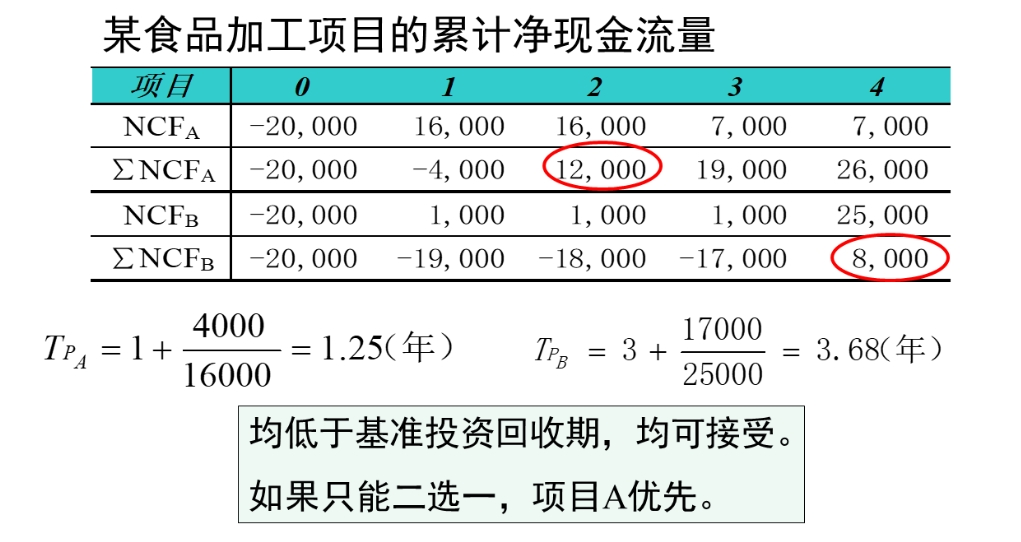
\includegraphics[width=\textwidth]{jxjll.png}
    \caption{例1:某食品加工项目的累计净现金流量}
    \label{fig:1}
\end{figure}

\subsection{指标评价}
\textbf{缺点}
\begin{itemize}
    \item 没有反映资金的时间价值;
    \item 未考虑回收期后的现金流,不能反映项目在整个投资期内的真实收益;
    \item 基准投资回收期的确定具有主观性。
\end{itemize}

\textbf{优点}
\begin{itemize}
    \item 简单、易懂;
    \item 在一定程度上反映了项目的经济性和风险大小。
\end{itemize}

\section{投资收益率(Return on investment)}

\subsection{总投资收益率(ROI)}

项目正常年份的息税前利润与投资总额的比值。
$$ROI=\mbox{息税前利润/总投资经济}$$

含义:项目投产后单位投资所创造的收益额。

\subsection{项目资本金净利润率(ROE)}

项目正常年份的年净利润与项目资本金的比值。
$$ROI=\frac{\mbox{净利润}}{\mbox{资本金经济}}$$

含义:项目投产后单位资本金所创造的收益额。

案例:
\begin{figure}[H]
    \centering
    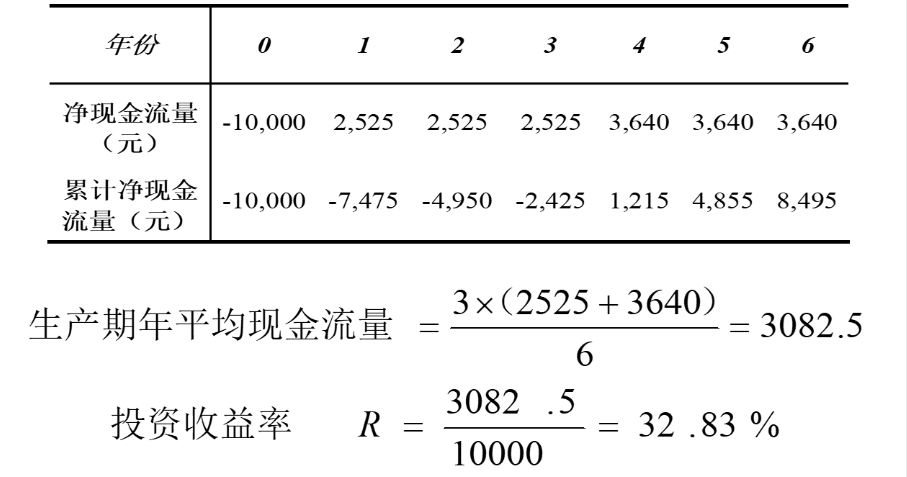
\includegraphics[width=\textwidth]{image/roi.png}
    \caption{例2:投资收益率}
    \label{fig:2}
\end{figure}

\subsection{判别准则}
设基准投资收益率为 $R$:
\begin{itemize}
    \item 若$R \geq R_b$,则项目可以考虑接受;
    \item 若$R \textless R_b$,则项目应予以拒绝。
\end{itemize}

\subsection{缺点}
\begin{itemize}
    \item 没有考虑时间价值;
    \item 当项目各年的经营状况不稳定时,该指标难以应用。
\end{itemize}

静态评价指标主要使用于\textbf{寿命周期较短且每期现金流量分布均匀}的技术方案评价,方案初选阶段。

\section{净现值(Net present value, NPV)}

\subsection{概念}
按一定的折现率将各年的净现金流量折现到期初的现值之和,反映项目净收益的现值。
\subsection{计算公式}
(不建议直接理解公式,建议跳过该部分,看例题)

$$NPV=\sum_{t=0}^{n}(CI-CO)_t(1+i_0)^{-t}=\sum_{t=0}^{n}NCF_t(1+i_0)^{-t}$$

\subsection{例题}
某工程项目总投资为5000万元,项目寿命期为10年,投资后1-10年内每年末可带来800万元的现金净流入,在10年末,还能回收资金200万元,基准折现率为12%,求项目的净现值,并判断该项目是否可行?\\
\textbf{答案:}$NPV = −5000 +800(P / A,12\%,10) + 200(P / F,12\%,10)= −415.60$(万元)

其中,$-5000$ 为现金流出现值,$800(P / A,12\%,10) + 200(P / F,12\%,10)$为现金流入现值。

那么,如何理解最后算得的结果呢?

算得的NPV值为$-415.60 \textless 0$,这表明如果投资该方案,则由该方案所带来的未来收益的现值小于现在投资的现值,即在一定折现率的条件下,未来收益不能全部回收现在的投资,项目在经济上不可行。

\subsection{判别标准}
若是一个方案,想要知道它可不可行,只需要把它的NPV值与0进行比较,若大于等于0则可行,小于0则不可行;而若是多个方案,只需要比较NPV值的大小,NPV值越大相对方案越优。

\subsection{确定项目的技术经济边界}
利用盈亏平衡原理的思路,可以根据决策需要建立技术经济边界分析模型(NPV=0),从技术角度反映经济问题。当项目盈亏平衡时,诸多影响项目技术经济效益的变量都存在一个临界值,即技术经济边界,合理确定这些边界将有利于项目的科学决策。

一个例子,上例中的变化基准折现率和净现值的计算,表格如下:
\begin{figure}[H]
    \centering
    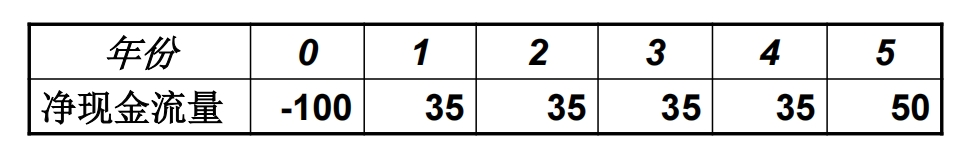
\includegraphics[width=0.9\textwidth]{image/年份-净现金流量.png}
    \label{fig:13}
\end{figure}
\begin{figure}[H]
    \centering
    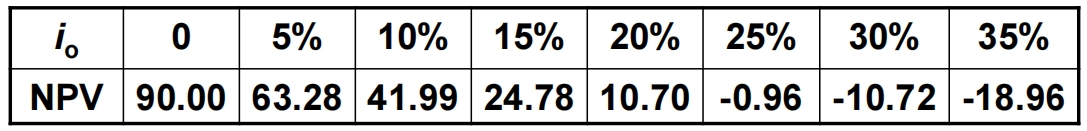
\includegraphics[width=0.9\textwidth]{image/i0-NPV.png}
    \label{fig:14}
\end{figure}

\begin{figure}[H]
    \centering
    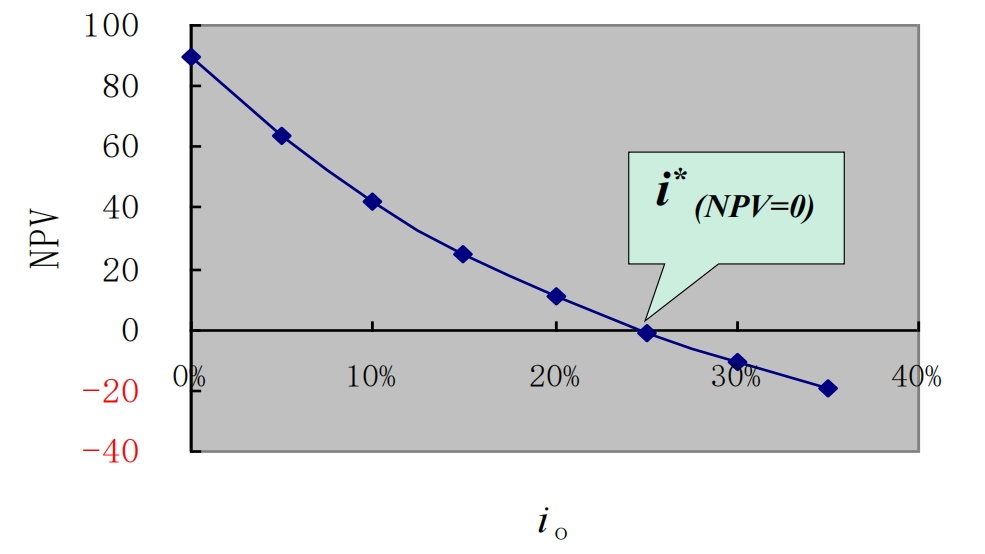
\includegraphics[width=\textwidth]{image/净现值与基准折现率的关系图示.png}
    \caption{净现值与基准折现率的关系图示}
    \label{fig:15}
\end{figure}

\textbf{净现值函数的特点:}同一净现金流量的净现值NPV随基准折现率$i_0$的增大而减小;基准折现率$i_0$定的越高,方案越可能被拒绝。

$i*$ 为折现率临界值,此时 NPV = 0;

i \textless i * 时, NPV \textless 0;

i \textgreater i * 时, NPV \textgreater 0。

\subsection{净现值对折现率的敏感性问题}
\subsubsection{举例}
下表列示了两个相互排斥的方案A、B的净现金流量,及其在折现率分别为10\%和20\%时的净现值。

\begin{table}[H]
\centering
\begin{tabular}{|c|c|c|c|c|c|c|c|c|}
\hline
    & 0   & 1   & 2   & 3   & 4   & 5   & NPV (10\%) & NPV (20\%) \\ \hline
A   & -230 & 100 & 100 & 100 & 50  & 50  & 83.91      & 24.81      \\ \hline
B   & -100 & 30  & 30  & 60  & 60  & 60  & 75.40      & 33.58      \\ \hline
\end{tabular}
\end{table}

当i=10\%时,$NPV_A \textgreater NPV_B$,则方案A优于方案B;

当i=20\%时,$NPV_A \textless NPV_B$,则方案B优于方案A。

此外,由表格后两列可以看出,方案A的净现值对折现率更敏感。

此现象,对投资决策的意义:

假设在一定的$i_0$和投资总限额$K_0$下,净现值大于0的项目有5个,其投资总额恰为$K_0$,故上述项目均被接受。按NPV的大小,其排序为A、B、C、D、E。

但若现在的投资总额必须压缩,减至$K_1$时,新选项目是否依然会遵循原排列顺序A、B、C...直至达到投资总额为止呢?一般说不会。

随着投资总额的压缩,应当提高基准折现率,但基准折现率由$i_0$提高到$i_1$后,由于各项目方案净现值对i的敏感性不同,原先净现值小的项目,其净现值现在可能大于原先净现值大的项目。

\section{净现值指数(Net present value index, NPVI)}
\subsection{概念}
项目的净现值与项目投资的现值之比。
\subsection{计算公式}
$$NPVI=\frac{NPV}{K_P}=\frac{NPV}{\sum_{t=0}^{n}K_t(1+i_0)^{-t}}$$

一个没见过的概念,$K_P$:项目投资现值。

NPV:考察的是资金利用的效果(绝对数),即总投资所能带来的净现值;

NPVI:可以考察资金利用的效率(相对比率),即单位投资所能带来的净现值。(排除了不同项目投资规模不同的影响)

\subsection{判别准则}
\noindent{\textbf{单一项目方案而言(与净现值相同)}:}

若NPVI \textgreater 0,则项目应予以接受;若NPVI \textless 0,则项目应予以拒绝。\\
\textbf{多方案比选时}:

净现值最大准则:NPV越大的方案相对越优。

注意:多方案比选时,NPV最大的方案,其NPVI不一定最大,此时,应根据NPV指标进行判断,选取NPV大的方案。简单理解:投资者追求的目标为在同等风险条件下获取的盈利最大。而净现值指标就是反映这种盈利的指标。\\
\textbf{例题:}项目各年净现金流量如下所示,基准折现率i=10\%,计算NPVI。
\begin{table}[H]
\centering
\begin{tabular}{|c|c|c|c|c|c|c|c|c|c|}
\hline
t   & 0 & 1 & 2 & 3 & 4  & 5  & 6  & 7   & 8      \\ \hline
NCF   & -100 & 50  & 45  & 45  & 45  & 45  & 45  & 45  & 45     \\ \hline
\end{tabular}
\end{table}
\textbf{答案:}$NPV =-100-50(P/F,10\%,1)+45(P/A,10\%,7)(P/F,10\%,1)=53.71$
$$NPVI=\frac{53.71}{100 50(P/F,10\%,1)}=0.37$$

\section{净年值(NAV)}

\subsection{概念}
通过资金等值换算,将项目净现值分摊到寿命期内各年的等额年值。
\subsection{公式}
$$NAV=NPV(A/P,I,N)$$
\subsection{判别标准}
对于单独一个项目:

$NAV \geq 0$:接受

NAV \textless 0:拒绝

就项目的评价结论而言,NPV,NAV是等效评价指标。\\
\textbf{例1:}某厂拟购置一台设备,购置费为100万元,预计使用五年后残值为20万元,在使用期5年内,由于使用这台机器每年可得收入50万元,而每年维修费等支出为22万元,若基准收益率为10\%,则净年值为?\\
\textbf{答案:}
\begin{figure}[H]
    \centering
    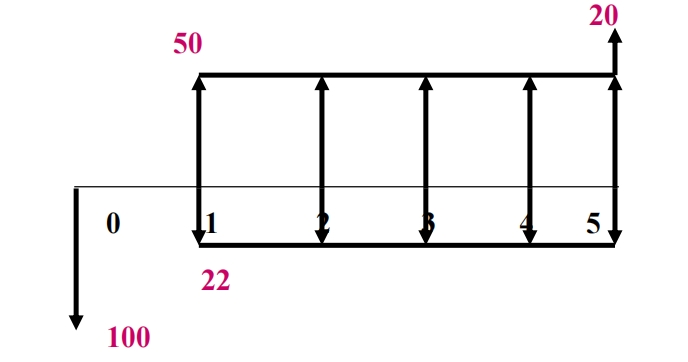
\includegraphics[width=0.7\textwidth]{image/NAV例题.png}
    \label{fig:16}
\end{figure}
\noindent{$NAV(10\%) = - 100(A/P,10\%,5)+28+20(A/F,10\%,5)= - 26.38 + 28 + 3.28= 4.9 \textgreater 0$}\\
$\because NAV(10\%) \textgreater 0$, \\
$\therefore$ 值得购置。\\
\textbf{例2:}(多选)关于净现值指数和净年值指标,说法正确的是(  )\\
A. 某方案,若净现值大于0,则净现值指数也大于0\\
B. 净现值指数是指单位投资现值所能带来的净现值\\
C. 多方案比较时,净现值指数可以作为净现值的辅助评价指标\\
D. 净年值体现项目生产期内每年的等额的超额收益\\
\textbf{答案:}ABC

\section{费用现值(PC)与费用年值(AC)}
\subsection{适用范围}
在对\textbf{多个方案}比较选优时,如果诸方案\textbf{产出价值相同},或者诸方案能够满足同样需要,其产出效益\textbf{难以用价值形态(货币)衡量}时,可以通过对各方案费用现值或费用年值比较进行选择。

\subsection{计算公式}
\subsubsection{费用现值的表达式:}
$$PC=\sum_{t=0}^{n}CO_{t}(P/F,i_0,t)$$

\subsubsection{费用年值表达式:}
$$AC=PC(A/P,i_0,n)=\sum_{t=0}^{n}CO_{t}(P/F,i_0,t)(A/P,i_0,n)$$

\subsection{判断准则}
费用现值和费用年值指标只能用于多个方案的比选,\textbf{费用现值或费用年值最小}的方案为优。

费用现值和费用年值的关系,与前述净现值和净年值的关系一样,故就评价结论而言,二者是等效评价指标。

\textbf{注意:PC与AC不能评价项目是否可行,只能用于多方案选优。}\\
\textbf{例1:}有两台功能相同、但费用不同的设备,试分析应选购哪台设备?(单位:万元,$i_0 = 15\%$)

\begin{table}[H]
\centering
\begin{tabular}{|c|c|c|c|c|}
\hline
设备 & 购置费用 & \multicolumn{2}{c|}{年运行费} & 第6年末残值 \\ \hline
    &           & 前3年每年 & 后3年每年 &              \\ \hline
A   & 10        & 5         & 6         & 4            \\ \hline
B   & 7.5       & 6         & 6         & 0            \\ \hline
\end{tabular}
\caption{设备购置及年运行费用和残值表}
\end{table}

\noindent{\textbf{答案:}}\\
$AC_A(15\%) = 10(A/P,15\%,6) + 5 + [1(F/A,15\%,3) – 4](A/F,15\%,6)= 7.58$(万元)\\
$AC_B(15\%) = 7.5 (A/P,15\%,6) + 6 = 7.98$(万元)\\
$\because AC_A(15\%) < AC_B(15\%)$,\\
$\therefore$ 应选择A设备;\\
$PC_A(15\%)=7.58 (P/A,15\%,6) =7.58×3.784=28.68$(万元)\\
$PC_B(15\%)=7.98 (P/A,15\%,6) =7.98×3.784=30.20$(万元)\\
$\because PC_A(15\%) < PC_B(15\%)$\\
$\therefore$ 应选择A设备。\\
\textbf{例2:}关于PC、AC指标,说法错误的是( )\\
A. PC、AC的指标值一般都小于0\\
B. PC、AC可用于单一方案的评判\\
C. 利用PC、AC指标时,可不考虑残值收入\\
D. PC、AC评判寿命期相等的方案时,是等效的\\
\textbf{答案:}ABC

\section{内部收益率(Internal rate of return, IRR)}
\subsection{概念}
净现值为零时的折现率(IRR)。
\begin{figure}[H]
    \centering
    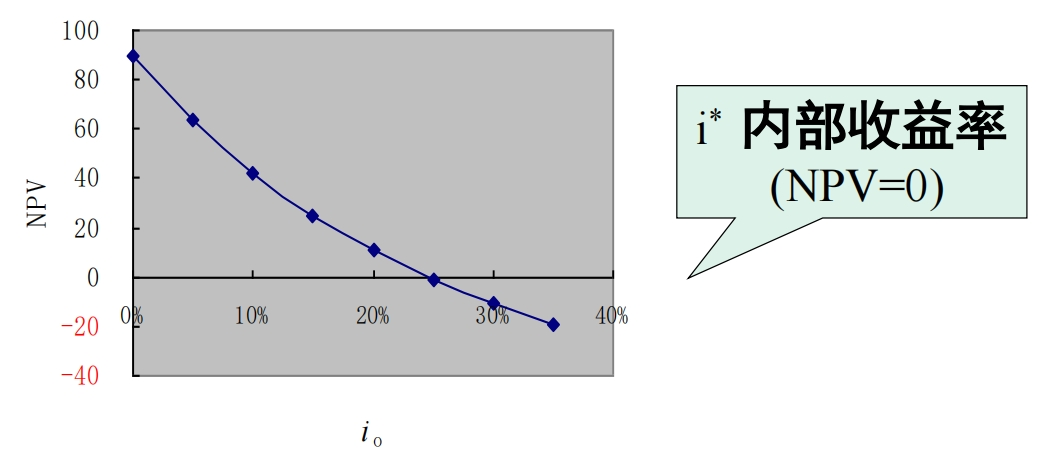
\includegraphics[width=\textwidth]{image/内部收益率IRR.png}
    \label{fig:17}
\end{figure}

\subsection{计算公式}
此处略,因为一元高次方程解起来太复杂,所以直接看例题,学会使用“试算内插法”即可。

\subsection{内部收益率计算的试插法}
\begin{figure}[H]
    \centering
    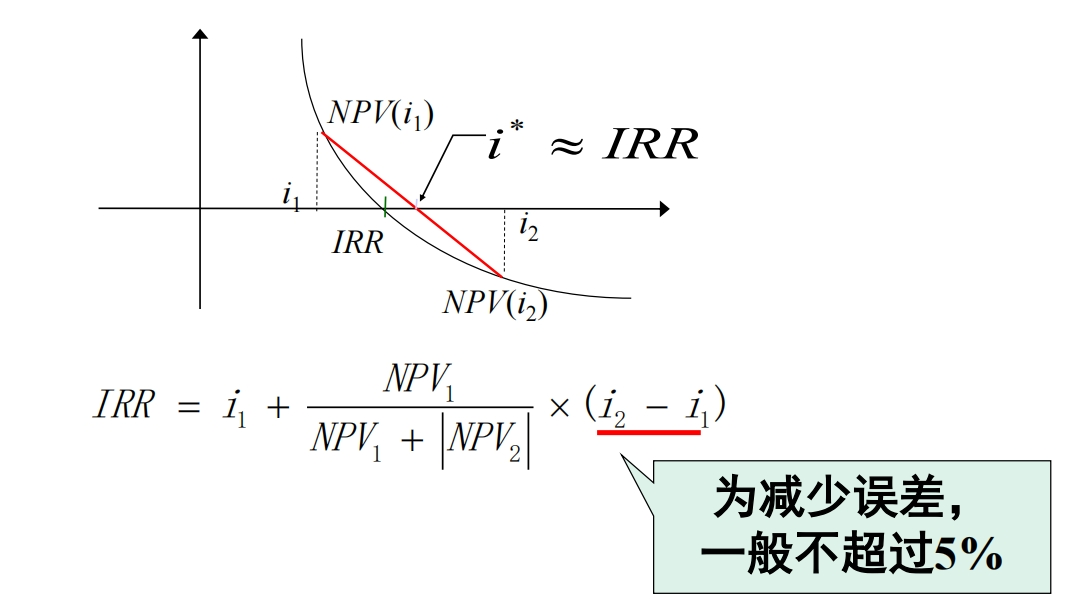
\includegraphics[width=0.9\textwidth]{image/试算内插法.png}
    \label{fig:18}
\end{figure}

\noindent{\textbf{例1:}}
\begin{table}[H]
\centering
\begin{tabular}{|c|c|c|c|c|c|c|}
\hline
t   & 0 & 1 & 2 & 3 & 4  & 5  \\ \hline
NCF   & -20000 & 6000  & 6000  & 7000  & 7000  & 10000   \\ \hline
\end{tabular}
\end{table}
\noindent{\textbf{答案:}}\\
$NPV = −20000 + 6000(P/ A,i,2) + 7000(P/ A,i,2)(P/ F,i,2) +10000(P/ F,i,5) = 0$\\
$i_1=20\%, NPV_1=612$\\ 
$i_2=25\%, NPV_2=-1632$
$$IRR=20\%+\frac{612-0}{612-(-1632)} \times 5\%=21.36\%$$
21.26\%就是项目自身的收益率。\\
\textbf{例2:}
\begin{table}[H]
\centering
\begin{tabular}{|c|c|c|c|c|c|c|}
\hline
t   & 0 & 1 & 2 & 3 & 4  & 5  \\ \hline
NCF   & -20000 & 7800  & 7800  & 7800  & 7800  & 7800   \\ \hline
\end{tabular}
\end{table}
\noindent{\textbf{答案:}}\\
$NPV = −20000 + 7800(P/ A,IRR,5) = 0$\\
$(P/A,IRR,5) = 2.5641$\\
\textbf{试插:}\\
$(P/A,25\%,5)=2.6893$\\
$(P/A,30\%,5)=2.4356$
$$IRR=25\%+\frac{2.6893-2.5641}{2.6893-2.4356} \times 5\% =27.47\%$$

\subsection{判别准则($i_0$为基准折现率/收益率/贴现率)}
$IRR \geq i_0$,项目可以接受;
$IRR \textless i_0$ ,项目应该拒绝。

基准收益率是投资者要求的最低投资收益率,如果项目的收益率大于或等于基准收益率,则项目经济可行;如果项目的收益率低于基准收益率,则项目不经济。

对某一方案而言:$IRR \geq i_0$, 即$NPV \geq 0$ ;$IRR \textless i_0$,即$NPV \textless 0$

\subsection{内部收益率隐含的经济意义}
\noindent{\textbf{表述一:}}

在项目的整个寿命期内,按利率i*=IRR来计算,会始终存在未能收回的投资,只有在寿命期结束时,投资恰好被全部收回。即在项目寿命期内,项目始终处于“偿付”未被收回的投资的状况。\\
\textbf{表述二:}

IRR是项目寿命期内没有回收投资的盈利率。\\
\textbf{例1:}
\begin{table}[H]
\centering
\begin{tabular}{|c|c|c|c|c|c|c|}
\hline
t   & 0 & 1 & 2 & 3 & 4  & 5  \\ \hline
NCF   & -20000 & 7800  & 7800  & 7800  & 7800  & 7800   \\ \hline
\end{tabular}
\end{table}
其IRR=27.47\%。当以IRR为折现率时,一直到项目寿命期末,才将未收回的投资全部回收。当以IRR为折现率时,可求得该投资项目在寿命期内,对应于每一年的净现值。\\
\textbf{例2:}某公司购买一台设备投资100000万元,寿命期为4年,每年年末的净收益分别是40000,37000,24000,22000元,可求得内部收益率等于10\%。它表示在寿命期内未被收回的投资在10\%的利率下,项目寿命期终了时能被完全收回。

内部收益率指标是一个相对指标,未考虑投资规模等对投资决策的影响,因此有时会做出错误的选择。如:投资期内项目净现金流入多次改变符号时、投资项目初始投资额不等时、投资项目现金流量发生的时间不同时。

\section{动态投资回收期}
\subsection{概念}
指项目累积净现金流量现值为零所需要的时间。(克服静态投资回收期未考虑资金时间价值的缺点)

\subsection{计算公式}
$$\sum_{t=0}^{T_P}(CI-CO)_t(1+i_0)^{-t}=0$$

\subsection{判别准则}
设Tb*为基准动态投资回收期,
若TP* $\leq$ Tb*,则项目可以考虑接受;
若TP* $\textgreater$ Tb*,则项目应予以拒绝。


\chapter{经济效果评价方法}
决策对象只有一个方案时,则可用NPV、IRR等指标评价标准进行该方案的选取。当决策对象存在多个方案需要进行选取时,孰优孰劣?需要依据其决策结构的不同而选用不同方法。多个方案之间的关系:独立方案、互斥方案、相关方案。

\section{独立方案的经济效果评价}
\subsection{概念-独立方案}
作为评价对象的各个方案的现金流是独立的,不具有相关性,且任一方案的采用与否都不影响其他方案是否采用的决策。

\subsection{独立方案的评价}
独立方案的采用与否,只取决于方案自身的经济性,即只需检验各个方案能否通过NPV、NAV、IRR等指标的评价标准。

\textbf{“绝对经济效果检验”}

\subsection{举例:}两个独立方案A和B,其现金流如表所示,试判断其经济性($i_0$=15\%)

\begin{table}[H]
\centering
\begin{tabular}{|c|c|c|}
\hline
t   & 0 & 1-10  \\ \hline
A   & -200 & 45 \\ \hline
B   & -200 & 30 \\ \hline
\end{tabular}
\caption{独立方案A、B的净现金流量(单位:万元)}
\end{table}
\noindent{\textbf{答案:}\\
(1)本例为独立方案,先计算方案自身的绝对效果指标,NPV、或者 NAV、IRR,再进行判断。}\\
$NPV_A=-200+45(P/A,15\%,10)=25.8$万元\\
$NPV_B=-200+30(P/A,15\%,10)=-49.4$万元\\
按NPV判断标准, $NPV_A  \textgreater 0$, $NPV_B \textless 0$,所以A方案予以接受,B方案应予拒绝。\\
(2) $NAV_A= NPV_A(A/P,15\%,10)=-200(A/P,15\%,10)+45=5.14$万元\\
$NAV_B= NPV_B(A/P,15\%,10)=-200(A/P,15\%,10)+30=-9.85$万元\\
按NAV判断准则,$NAVA \textgreater 0$, $NAVB \textless 0$,所以A方案予以接受,B方案应予拒绝。\\
(3)设A方案内部收益率为$IRR_A$,B方案内部收益率为$IRR_B$,由方程:\\
$$-200+45(P/A,IRR_A,10)=0$$
$$-200+30(P/A,IRR_B,10)=0$$
\noindent 解得:\\
$IRR_A=18.3\%,IRR_B=8.1\%,i_0=15\%$。据IRR判别标准,所以A予以接受,B拒绝。

\subsection{结论}
对于独立方案而言,经济上是否可行的判据是其绝对经济效果指标是否优于一定的检验标准。无论采用哪种评价指标,评价结论都是相同的。

\section{互斥方案的经济效果评价}
\subsection{概念-互斥方案}
方案之间存在互不相容、相互排斥关系的称为互斥方案,在对多个互斥方案进行比选时,至多只能选取其中之一。\textbf{“有你无我” 、“你死我活”}。
\subsection{互斥方案经济效果评价的内容}
一是考察各个方案自身的经济效果,即进行“绝对经济效果检验”;二是考察哪个方案相对最优,称“相对经济效果检验”。先看自身条件,再与候选比优!
\subsection{互斥方案经济效果评价特点}
要进行方案之间的比选;参加比选的方案之间应具有可比性。

如:考察时间段及计算期的可比性;方案风险水平的可比性;评价所使用假定的可比性。

\subsection{互斥方案的分类}
按互斥方案的寿命期是否相等,分为寿命期相等的互斥方案和寿命期不等的互斥方案。

\subsection{寿命期相等的互斥方案比选方法-增量分析法}
\subsubsection{引例}
由于理论不好直接理解,这里引入一个例子,从例子理解这个比选方法。\\
\textbf{例子:}互斥方案D、E的净现金流如下表所示,基准收益率为10\%,试判断应选择哪个方案?
\begin{table}[H]
\centering
\begin{tabular}{|c|c|c|}
\hline
年份   & 0 & 1-5  \\ \hline
方案D   & -100 & 35 \\ \hline
方案E   & -150 & 50 \\ \hline
\end{tabular}
\end{table}
\noindent{\textbf{解析:}}\\
(1)首先,进行“绝对经济效果检验”,计算两个方案的绝对经济效果指标NPV和IRR:
$NPV_D=-100+35 \times (P/A,10\%,5)=32.68$(万元)\\
$NPV_E=-150+50 \times (P/A,10\%,5)=39.54$(万元)\\
由方程:\\
$-100+35 \times (P/A,IRR_D,5)=0$\\
$-150+50 \times (P/A,IRR_E,5)=0$\\
解得: $IRR_D=22\%$,$IRR_E=20\%$\\
结论:方案D、E都能通过绝对经济效果检验。\\
(2)其次, 进行“相对经济效果检验”,按一定判别标准,比较哪个方案相对最优;\\
NPV法: $NPV_E \textgreater NPV_D$,若按NPV最大准则,方案E优于方案D;\\
IRR法: $IRR_E \textless IRR_D$。\\
若按IRR最大为比选准则,方案D优于方案E。\\
结论:以上采用不同指标,在一定评选准则下,进行相对评选,方案选择结果相互矛盾。

\textbf{矛盾的解决:}分析投资方案的本质在于增量投资的经济性。投资目的是获取最大收益,互斥方案的比选实际上是判断额外投资是否合理。较大投资的方案可分为两部分:第一部分与小投资方案相同,第二部分是增量投资的收益。如果增量投资的收益较好,则较大投资方案优;否则,小投资方案优。

\begin{table}[H]
\centering
\begin{tabular}{|c|c|c|}
\hline
年份   & 0 & 1-5  \\ \hline
方案D   & -100 & 35 \\ \hline
方案E   & -150 & 50 \\ \hline
差额现金流   & -50 & 15 \\ \hline
\end{tabular}
\end{table}

差额现金流即增量净现金流,通过ΔNCF,可以计算ΔNPV(增量净现值)或ΔIRR(增量内部收益率)。

差额投资收益是否满意的比选标准:ΔNPV>0,ΔIRR>$i_0$(单一方案比选标准)

上例中,ΔNPV=$-50+15(P/A,10\%,5)=NPV_E-NPV_D=39.54-32.68=6.86 \textgreater 0$

由方程-50+15(P/A,ΔIRR,5)=0可解得ΔIRR=15.2\%>10\%

相对比选结论:E优(增量投资有满意的增量收益)

最终结论:E优(同时通过绝对/相对经济效果检验)

\subsubsection{概念-增量分析法}
通过计算ΔNCF(增量净现金流)的经济效果评价指标ΔNPV(增量净现值)、ΔIRR(增量内部收益率)等来评价增量投资经济效果,从而对\textbf{投资额不等的互斥方案}进行比选的方法,称为\textbf{增量分析法(差额分析法)}(互斥方案比选的基本方法)。

在对互斥方案进行比选时,分别用ΔNPV 、 ΔIRR 、NPV(最大)、 NAV(最大)、 PC、AC(最小)、等指标的判别准则进行方案选优时,结论是一致的,正确的;但IRR最大准则,不能总保证比选结论的正确性。当ΔIRR \textless $i_0$,IRR最大准则成立;ΔIRR ≥ $i_0$, IRR最大准则不成立。

\section{寿命期不等的互斥方案比选方法}
绝对经济效果检验:可采用净现值法
如何进行相对比较?假设各方案可以按原有规模不断重复。以互斥方案寿命期最小公倍数作为比较期,最短计算期法,以互斥方案无限循环期作为比较期,以一年作为比较期。

\textbf{年值法-最简便(避免“期”不同问题)}\\
NAV(净年值):最大且非负为最优方案;\\
AC(费用年值):最小为最优方案。

\textbf{年值折现法-设定共同分析(计算)期}\\
首先将各个方案的年值按某一共同的分析期折现,得到用于方案比选的现值(净现值/费用现值)。再根据净现值/费用现值的比选准则进行方案选取。

\section{相关方案比较(了解即可)}
在多方案之间,如果接受(或拒绝)某一方案,会显著改变其他方案的现金流量,或会影响其他方案的接受(或拒绝),就说这些方案是相关的。

\subsection{种类}
\textbf{1、完全互斥型:}\\
接受某一方案,就必须放弃其他方案。“有你无我”(在前面已经有详细的讲解)

\textbf{2、相互依存型和完全互补型}\\
含义:如果两个或多个方案之间,某个方案的实施要求以另一方案(或另几个方案)的实施为条件,则这两个方案(或若干个)方案具有相互依存性,或者说具有完全互补性。

举例:在两个不同的军工厂分别建设生产新型火炮和与之配套的炮弹的项目。

\textbf{3、现金流相关型}\\
含义:如果若干方案中,任一方案的取舍会导致其他方案现金流的变化,则这些方案之间为现金流相关型。

举例:A方案是在某大河上建一座收费公路桥,B方案是在桥址附近建收费轮渡码头,任一方案的实施或放弃都会影响另一方案的收入。

\textbf{4、资金约束导致的方案相关}\\
含义:在资金有限的情况下,接收某些方案则意味着不得不放弃另外一些方案。

\textbf{5、混合相关型}\\
含义:在方案众多的情况下,方案间的相互关系可能包括多种类型,称为混合相关型。

\section{本章重点总结}

\subsection{独立方案决策}
NPV $\geq 0$、IRR $\geq i_0$

\subsection{互斥方案决策(最为重要)}
\subsubsection{1. 收益现金流项目}
\textbf{(1)寿命期相等:重要}
\begin{itemize}
    \item 选择NPV $\geq 0$,且NPV最大的项目;
    \item 如果IRR $ \geq i_0$,则选择投资额较大的项目;如果IRR $< i_0$,则选择投资额较小的项目。
\end{itemize}

\textbf{(2)寿命期不等:}
\begin{itemize}
    \item \textbf{年值法:选择NAV最大且大于零的项目;重要}
    \item 寿命期最小公倍数法:选择NPV(N)最大且大于零的项目;
    \item 无限循环法:选择NPV大于零,且NPV最大的方案。
\end{itemize}

\subsubsection{2. 费用现金流项目}
\textbf{(1)寿命期相等:}

\textbf{选择PC或AC最小的项目。重要}

\textbf{(2)寿命期不等:}
\begin{itemize}
    \item 选择寿命期最小公倍数内PC最小的项目;
    \item 选择AC最小的项目。重要
\end{itemize}

\subsection{现金流相关方案决策(了解)}
\subsubsection{互斥方案组合法}
\subsection{资本限量决策(了解)}
\subsubsection{1. 互斥方案组合法}
\subsubsection{2. “净现值+剩余资金”法}
\chapter{不确定性分析和风险分析}
不确定性分析——通过对拟建项目具有较大影响的不确定性因素进行分析,计算基本变量的增减变化引起项目财务或经济效益指标的变化,找出最敏感的因素及其临界点,可以\textbf{预测项目可能承担的风险}。

通过不确定性分析可以找出\textbf{影响项目效益的敏感因素,确定敏感程度},但不知这种不确定性因素发生的可能性及影响程度,因而不能代替风险分析。

通过风险分析可以得到\textbf{不确定性因素发生的可能性以及给项目带来经济损失的程度}。

\section{盈亏平衡分析(Break-Even Analysis)}
\noindent\textbf{目的:}

找出各种不确定性因素变化的\textbf{临界值}(会影响方案取舍的数值),判断方案对不确定性因素变化的\textbf{风险承受能力},为决策提供依据。

\noindent{\textbf{种类-按是否考虑资金时间价值}}
\begin{figure}[H]
    \centering
    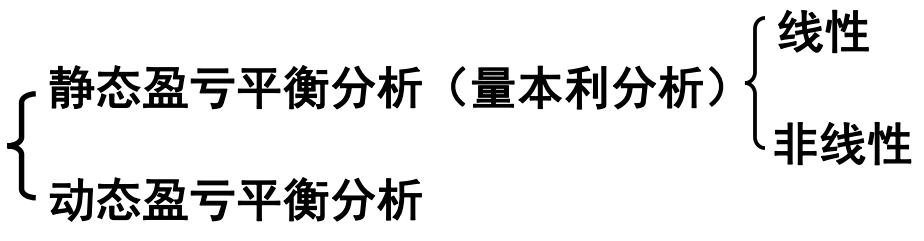
\includegraphics[width=0.7\textwidth]{image/盈亏平衡分析-种类.png}
    \label{fig:19}
\end{figure}

\subsection{线性静态盈亏平衡分析}
\subsubsection{含义}
分析\textbf{产量、成本与利润}之间的关系,找出投资方案\textbf{盈利或亏损}在产量、产品价格、单位产品成本等方面的\textbf{界限值},以判断在各种不确定因素作用下方案的风险状况(承受能力)。

\subsubsection{成本分类-按成本与产量的关系}
固定成本(Fixed costs, FC):在一定的产量范围内,\textbf{不随产量变动而变动}的成本。如设备折旧费等。

变动成本(Variable costs, VC):随产量的变动而变动的成本,如原材料等。通常假设变动成本与产量成正比关系,即:\textbf{变动成本 = 单位变动成本×产量}

\subsubsection{收入、成本、利润之间的关系}
1、年销售收入=价格×年产量=P×Q(假设销售价格不变,生产量=销售量)

2、年总成本=固定成本+变动成本=固定成本+单位变动成本×年产量=FC+v×Q 

3、年利润=年销售收入-年总成本= P×Q-(FC+v×Q)\\


\subsubsection{举例}
某投资项目需固定资产投资60万元,流动资金投资8万元,均在现在投入,项目当年建成投产,寿命期8年。项目的设计生产能力为生产产品10万件,预计价格7.5元/件,单位变动成本为4元/件,固定成本(未包括折旧)为每年10万元。假设项目固定资产投资全部形成固定资产原值,采用直线法折旧,折旧年限为8年,残值为0。

\textbf{原始资料:}
目前预计各参数数值:
\begin{itemize}
    \item 年设计生产能力10万件
    \item 产品价格7.5元/件
    \item 产品单位变动成本4.0元/件
    \item 固定成本:年折旧=60/8=7.5万元;年固定成本=10+7.5=17.5万元
\end{itemize}

根据上述资料,分别进行产量、价格、单位变动成本盈亏平衡点分析。\\
\textbf{1、产量盈亏平衡点分析}

在一定的价格、固定成本和单位变动成本下,使年利润为零的年产量。
$$P \times Q - (FC + v \times Q) = 0$$
$$Q^*=\frac{FC}{P-v}$$

若FC占总成本比例越大,则$Q^*$越高,即项目的风险性增大。

在本例中,$Q^*=\frac{17.5}{7.5-4.0}=5$(万件)

结论:
通过计算产量盈亏平衡点,可以对方案发生亏损的可能性作出大致判断。即项目的年产量只要达到或超过5万件,项目就不会亏损。

\begin{figure}[H]
    \centering
    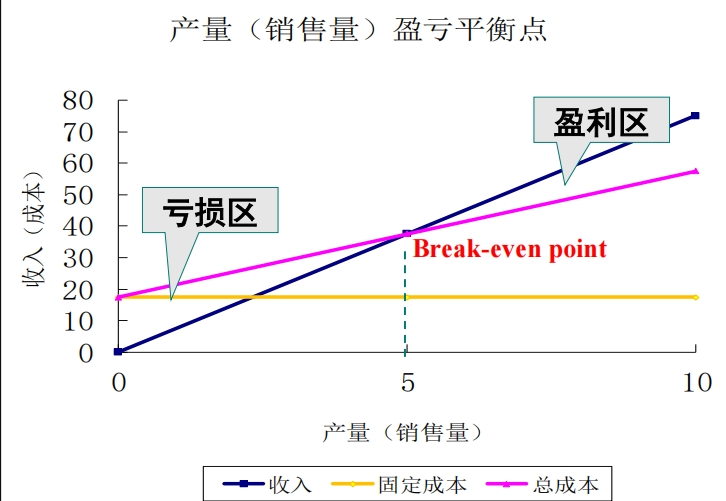
\includegraphics[width=0.75\textwidth]{image/盈亏平衡分析.png}
    \label{fig:20}
\end{figure}

盈亏平衡生产能力利用率:反映盈亏平衡产量占设计生产能力$Q_C$的比率。

$$E^*=\frac{Q^*}{Q_C} \times 100\% =\frac{5}{10} \times 100\% = 50\%$$

说明该项目年产量只要达到或超过设计生产能力的50\%,项目就不会亏损。\\\textbf{2、价格盈亏平衡点分析}

在固定成本和单位变动成本不变、按设计生产能力生产的情况下,使年利润为零的产品价格。

$P \times Q - (FC+v \times Q)=0$

$P* = \frac{FC}{Q_C}+v$

若FC占总成本比例越大,则$P^*$越高,即项目的风险性越大。

在本例中,$P^* = \frac{17.5}{10}+ 4.0 = 5.75$(元/件)

说明该项目产品的价格只要不低于5.75元/件,项目就不会亏损。

\begin{figure}[H]
    \centering
    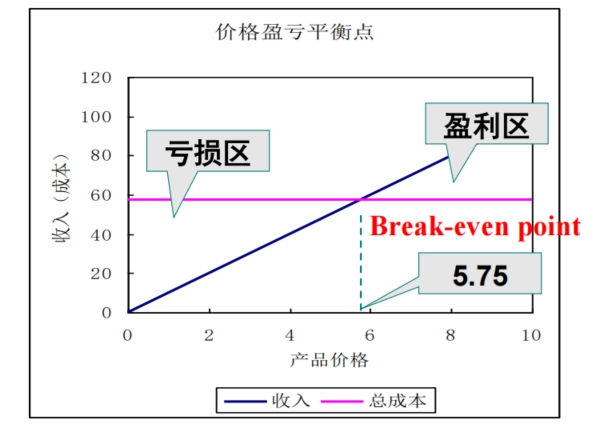
\includegraphics[width=0.75\textwidth]{image/静态盈亏平衡分析.png}
    \label{fig:21}
\end{figure}

\noindent \textbf{3. 单位变动成本盈亏平衡分析}

在产品价格和固定成本不变、按设计生产能力生产的情况下,使年利润为零的单位变动成本。

$P×Q-(FC+v×Q)=0$

$v^*=P-\frac{FC}{Q_C}$

若FC占总成本比例越大,则$V^*$越低,即项目的风险性越大。

在本例中,$v^*=7.5-\frac{17.5}{10}=5.75$(元/件)

说明该项目产品的单位变动成本只要不高于5.75元/件,项目就不会亏损。

\begin{figure}[H]
    \centering
    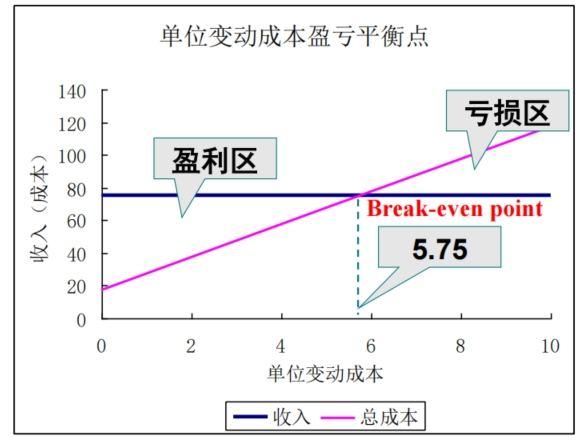
\includegraphics[width=0.75\textwidth]{image/单位变动成本盈亏平衡点.png}
    \label{fig:22}
\end{figure}

\subsubsection{成本结构与经营风险(自学范围,应该不考)}
理解结论的推导过程由销量及成本变动引起的经营风险的大小与项目固定成本占总成本费用的比例有关即可。

\subsubsection{静态盈亏平衡分析总结}
盈亏平衡分析的目的是找出临界值,即盈亏平衡点(BEP),判断投资方案对不确定因素变化的承受能力,为决策提供依据。

价格、产量盈亏平衡点越低,单位变动成本盈亏平衡点越高,说明项目盈利的可能性越大,亏损的可能性越小,因而项目有较大的抗经营风险能力。

\subsubsection{静态盈亏平衡分析的缺点}
(1)注重的是项目生产期的年利润,而没有考察项目的价值(没有考虑资金时间价值)。

(2)不适于分析生产期各年产量(销售量)不稳定的项目。

(3)分析较为笼统,只知道因素变化多大会使项目由盈利转为亏损。但因素的变化到底会使评价指标变化程度有多大还不知道。

\subsection{非线性静态盈亏平衡分析}
成本TC在实际中并不随产量呈直线变化,销售收入TR也受市场和用户的影响不呈线性变化。常见的是二次曲线型盈亏平衡分析。

\begin{figure}[H]
    \centering
    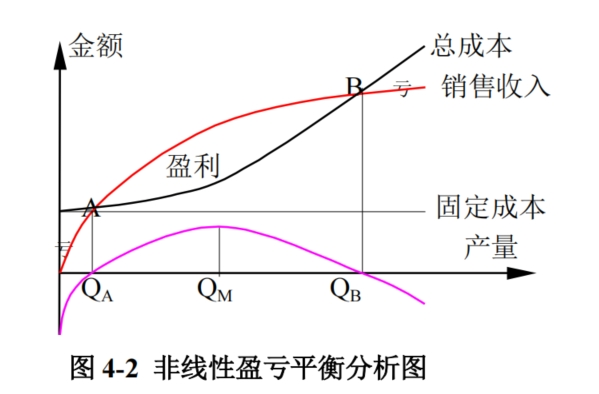
\includegraphics[width=0.7\textwidth]{image/非线性盈亏平衡分析图.png}
    \caption{非线性盈亏平衡分析图}
    \label{fig:23}
\end{figure}

设销售收入函数为f(x),成本函数为g(x),利润函数为 m(x)=f(x)-g(x)

解方程f(x)=g(x)得到的解为盈亏平衡时的产量。

令:

$$\frac{dm(x)}{d(x)}=\frac{d[f(x]-g(x)}{dx}=0$$

可得到最大利润所对应的产量$Q_M$及最大利润值。

例:某公司投资生产一种新产品,预计该产品的年销售收入$TR=3100Q-0.6Q^2$,年总成本$TC=3187500+600Q-0.2Q^2$。试求其盈亏平衡点的产量及利润最大化的产量。

当达到盈亏平衡点时,TR=TC,即:
$$3100Q-0.6Q^2=3187500+600Q-0.2Q^2$$
$$0.4Q^2-2500Q+3187500=0$$

\section{动态盈亏平衡分析}
\subsection{含义}
以项目的净现值为零,分析产量、价格、单位变动成本的变动临界点,从而判断项目在各种不确定因素作用下的风险状况。

即NPV=0时,分析

(1)在产品价格、单位变动成本、固定成本不变时,求年产量$Q^*$。

(2)在年产量为设计产量、单位变动成本和固定成本不变时,求产品价格$P^*$。

(3)在年产量为设计年产量、产品价格和固定成本不变时,求单位变动成本$v^*$。

\textbf{举例(原例续):}
某投资项目需固定资产投资60万元,流动资金投资8万元,均在现在投入,项目当年建成投产,寿命期为8年。项目的设计生产能力为生产某种产品10万件,预计产品价格为7.5元/件,单位变动成本为4元/件,固定成本(未包括折旧)为每年10万元。假设项目固定资产投资全部形成固定资产原值,采用直线法折旧,折旧年限为8年,残值为0。

\textbf{公司所得税税率为40\%,基准折现率为15\%。}(新增内容)

\textbf{解:}

初始现金流:-68万元

\noindent \textbf{营业现金流:}\\
收入:P×Q\\
变动成本:v×Q\\
固定成本:17.5万元\\
年利润:$(P-v)×Q-17.5$\\
年税后利润:$0.60 (P-v)×Q - 10.5$(年利润×0.6)\\
年营业现金流:$0.60 (P-v)×Q-3$(年利润+年折旧)

\begin{figure}[H]
    \centering
    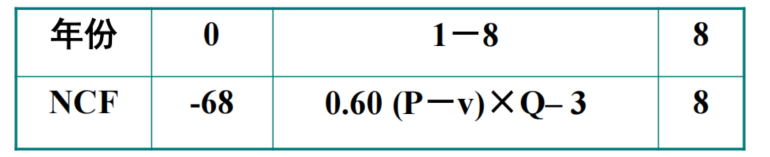
\includegraphics[width=0.75\linewidth]{image/表1.png}
\end{figure}

\noindent 令NPV = 0,
$$-68 +[0.60 \times (P − v) \times Q − 3](P/ A,15\%,8) + 8(P/ F,15\%,8) = 0$$
$$− 28.87 + (P −v) \times Q = 0$$
求得产量盈亏平衡点:8.24万件;价格盈亏平衡点:6.89元/件;单位变动成本盈亏平衡点:4.61元/件;终结现金流:8万元。

\noindent \textbf{结论:}

当产品价格为7.5元/件,单位变动成本为4.0元/件,年固定成本为17.5万元时,项目的年产量只要达到或超过8.24万件/年,或生产能力利用率达到或超过82.4\%,项目就有经济价值。

当项目按设计生产能力10万件/年进行生产,单位变动成本为4.0元/件,年固定成本为17.5万元时,产品价格只要达到或超过6.89元/件,项目就有经济价值。

当项目按设计生产能力10万件/年进行生产,产品价格为7.5元/件,年固定成本为17.5万元时,单位变动成本只要不超过4.61元/件,项目就有经济价值。

\noindent \textbf{例:}(单选)关于盈亏平衡分析,说法错误的是\\
A.盈亏平衡价格越高,项目的风险承受能力越高。\\
B.盈亏平衡产量越高,项目的风险承受能力越低。\\
C.盈亏平衡生产能力利用率越低,项目的风险承受能力越高。\\
D.固定投资占总成本比例越大,项目的风险性越大。\\
\textbf{答案:}A。

\section{敏感性分析}
\subsection{含义}
通过测定一个或多个不确定因素的\textbf{变化}所导致的决策评价指标的\textbf{变化幅度},了解各种因素的变化对实现预期目标的\textbf{影响程度},从而对外部条件发生不利变化时投资方案的\textbf{承受能力}作出判断。

\subsection{作用}
研究相关因素的变动引起经济效果评价指标的变动幅度;

找出敏感性因素,预测其可能产生的不确定性对方案的影响,以便采取控制措施;

敏感性分析结论有助于方案选优。

\subsection{种类:按所分析不确定性因素的个数}

\subsubsection{单因素敏感性分析(重点)}
假定其他因素不变,分析某一不确定因素的变动对方案经济效果产生的影响。\\
\textbf{(一)分析步骤}

1、选择需要分析的不确定因素,并设定这些因素的变动范围;

2、确定分析指标;

3、进行敏感性计算,建立敏感性分析表和分析图;

4、确定敏感因素,即其数值变动能显著影响方案经济效果的因素。

\noindent \textbf{(二)举例(续):}

假设上述投资项目中固定资产投资、产量、产品价格、单位变动成本等是不确定因素,这些因素都有可能偏离预计值-20\%到+20\%。分析哪些因素是敏感因素。

\begin{figure}[H]
    \centering
    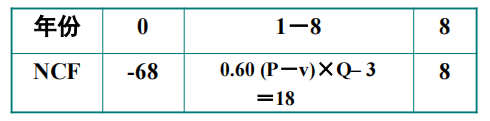
\includegraphics[width=0.85\linewidth]{image/单因素-例题.png}
\end{figure}

\textbf{1、基础方案}

固定资产投资60万元,流动资金投资8万元,年产量10万件,产品价格7.5元/件,单位变动成本4.0元/件,固定成本(不包含折旧)10万元/年,折旧7.5万元/年
$NPV=15.39$万元
$IRR=21.39\%$

\textbf{2、选定不确定因素,设定可能的变动范围}

固定资产投资、产量、产品价格、单位变动成本

变动范围为-20\%到+20\%

\textbf{3、确定分析的指标}:净现值NPV。

\textbf{4、敏感性计算及结果}

\begin{figure}[H]
    \centering
    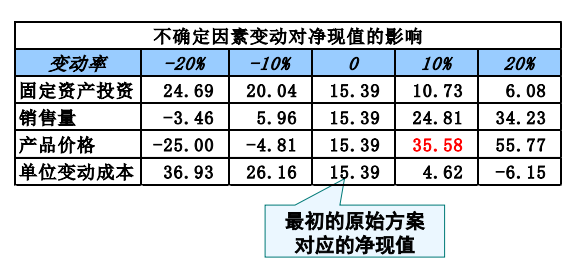
\includegraphics[width=1\linewidth]{image/不确定因素变动对净现值的影响.png}
\end{figure}

\begin{figure}[H]
    \centering
    \caption{产品价格变动10\%时,净现值的计算举例:}
    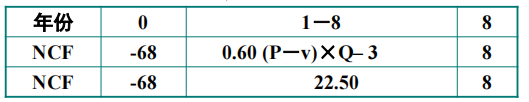
\includegraphics[width=0.85\linewidth]{image/净现值的计算举例.png}
\end{figure}

1-8年每年净现金流$= 0.60 (P-v) \times Q - 3 = 0.60 \times (7.5 \times 1.1 - 4) \times 10 - 3 = 22.50$

净现值$=-68+22.5 \times (P/A,15\%,8)+8 \times (P/F,15\%,8) = 35.58$

(目前预计价格7.5,产量10,单位变动成本4)

\begin{figure}[H]
    \centering
    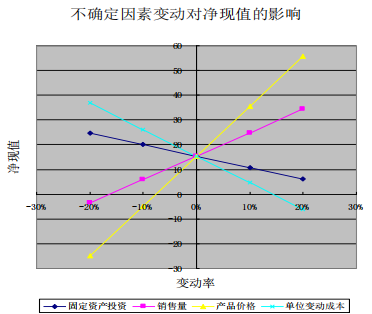
\includegraphics[width=0.8\linewidth]{image/敏感性计算及结果图示.png}
    \caption{敏感性计算及结果图示}
\end{figure}

\textbf{这个图很重要,斜率绝对值最大的对净现值影响最大。}

\textbf{5、判定敏感因素}

\noindent \textbf{相对测定法}

比较在同一变动幅度下各因素的变动,对经济效果指标产生的影响,据此判断方案经济效果对各因素变动的敏感程度。

\begin{figure}[H]
    \centering
    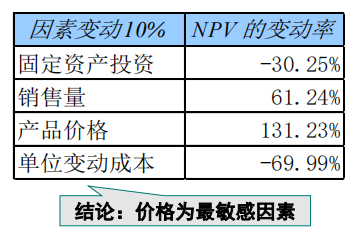
\includegraphics[width=0.75\linewidth]{image/相对测定法.png}
\end{figure}

\textbf{敏感度系数=项目评价指标变化率/不确定性因素变化率}

\noindent \textbf{绝对测定法}

测定使经济效果指标达到临界值时各因素的变动幅度,变动幅度越小,则方案的经济效果对该因素越敏感。

\begin{figure}[H]
    \centering
    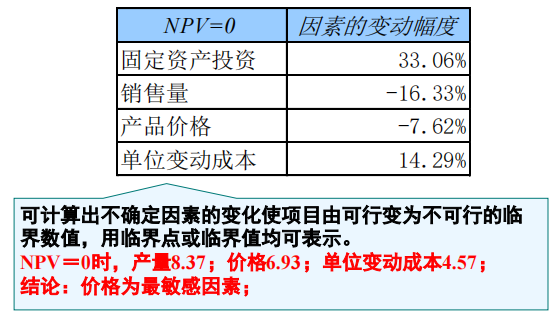
\includegraphics[width=0.75\linewidth]{image/绝对测定法.png}
\end{figure}

\textbf{例1:}(多选)关于敏感性分析,说法错误的是
A.单因素敏感性分析图中,影响因素直线斜率越小,该因素越敏感
B.比较在同一变动幅度下各因素的变动,对经济效果指标产生的影响越大,该因素越敏感
C.测定使经济效果指标达到临界值时各因素的变动幅度,变动幅度越小,该因素越敏感
D.敏感性分析没有考虑各种不确定性因素在未来发生变动的概率

\textbf{例2:}单因素敏感性分析中,甲、乙、丙、丁四因素分别发生5\%、10\%、10\%、15\%的变动,经济效果评价指标均发生20\%的变动,最敏感的因素是?

\textbf{答案:}甲。



\subsubsection{多因素敏感性分析(不重要)}
分析多个因素同时变动对方案经济效果的影响。

\noindent \textbf{1.引入-单因素敏感性分析的局限性}

单因素敏感性分析,计算某一因素变动对经济效果指标的影响时,假定其他因素均不变。

但实际上,一个因素的变动往往也伴随着其他因素的变动。

如:产品价格上涨时,产品需求量可能下降。

解决方法:引入多因素敏感性分析。

\noindent \textbf{2.特点:}

多因素敏感性分析需要考虑可能发生的各种因素不同变动幅度的多种组合,计算起来相对复杂的多。

如果需要分析的不确定性因素不超过三个,可以用解析法和作图法相结合的方法进行。

\subsection{敏感性分析评价}
敏感性分析在一定程度上,就各种不确定性因素的变动对经济效果的影响作了定量描述。有助于帮助确定在决策过程中,需要重点研究和控制的因素。

但敏感性分析没有考虑各种不确定性因素在未来发生变动的概率,可能会影响分析结论的正确性。

如通过敏感性分析找出的某一敏感因素,在未来发生不利变动的概率很小,因而实际上所带来的风险并不大。

解决办法:进行概率分析。

\section{概率分析}
看看得了,我觉得不考。

\section{风险决策(理解决策原则)}
\subsection{引入}
概率分析可以给出方案经济效果指标的期望值和标准差,以及指标的实际值发生在某一区间的概率。但是概率分析没有给出风险条件下,方案取舍的原
则和多方案比选的方法。

\subsection{风险决策条件}
1、存在着两个或两个以上可供选择的方案;

2、存在两种或两种以上的随机自然状态;

3、已知各种自然状态出现的概率;

4、已知各种自然状态下,各方案经济效果指标的估值;

5、存在着决策人希望达到的目标(收益最大/损失最小)

\subsection{举例}
某企业拟开发一种新产品取代将要滞销的老产品。技术部门提出了三种方案,新产品投入市场后可能出现四种前景。已经估计了每种前景出现的概率,各方案在每种前景下可能的净现值,决策者要解决的问题是应该选择哪个方案。

\begin{figure}[H]
    \centering
    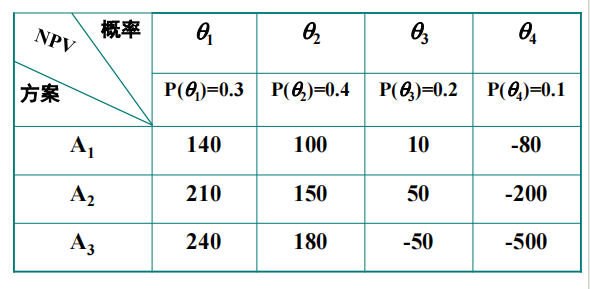
\includegraphics[width=0.75\linewidth]{image/风险决策-选哪个方案.png}
\end{figure}

\subsection{风险决策原则(可能考选择或简答)}
优势原则、期望值原则、最小方差原则、最大可能原则、满意原则。

\subsubsection{(1)优势原则}
在互斥方案A、B中,如果不论在什么状态下A总是优于B,则可以认定A相对于B是优势方案,从而剔除B。

应用优势原则一般不能决定最佳方案,但能够减少备选方案的数目。

在采用其他决策原则进行方案比选之前,应首先运用优势原则剔除劣势方案。

\subsubsection{(2)期望值原则}
选择净现值的期望值最大的方案,或费用现值的期望值最小的方案。

在上例中,按照期望值原则应选择A2。

$E(NPV)1=76$万元

$E(NPV)2=113$万元

$E(NPV)3=84$万元

\subsubsection{(3)方差最小原则}
选经济效果指标的方差最小的方案。

在上例中,按照方差最小原则应选择A1。

$D(NPV)1=4764$万元

$D(NPV)2=13961$万元

$D(NPV)3=48684$万元

与期望值原则得出的结论不同。

\subsubsection{(4)最大可能原则}
如果一种状态发生的概率显著大于其他状态,那么就把这种状态视作肯定状态,根据这种状态下各方案的经济效果指标来进行决策。

按照最大可能原则决策实际上将风险决策问题转化为确定性决策问题。

\noindent \textbf{注意:适用前提:}

1、一种状态发生的概率显著大于其他状态;

2、各方案在不同状态下的损益值的差别不很悬殊;

\textbf{按最大可能原则分析上例:}

状态$\theta 2$发生的概率最大,如果按照最大可能原则决策,应选择$\theta 2$下净现值最大的A3方案。

\begin{figure}[H]
    \centering
    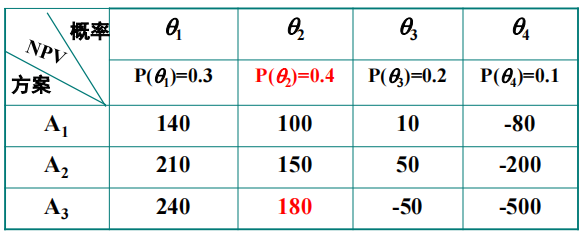
\includegraphics[width=0.75\linewidth]{image/最大可能原则分析.png}
\end{figure}

但从本例的适用前提来看,

$\theta 2$发生的概率P($\theta 2$)=0.4,与其他状态发生的
概率差别不大;A3方案在不同状态下净现值相差较大。

即最大可能原则在本例中不太适用。

\noindent\textbf{(5)满意原则}
定出一个足够满意的目标值,将各备选方案在不同状态下的经济效果指标与此目标值进行比较,选择经济效果指标优于或等于目标值的概率最大的方案。

上例中如果满意目标是净现值不小于30万元,则应该选择A2。

P(NPV $\geq$ 30)1=P($\theta 1$)+ P($\theta2$)=0.7

P(NPV $\geq$ 30)2= P($\theta 1$)+ P($\theta2$) + P($\theta3$) =0.9

P(NPV $\geq$ 30)3=P($\theta 1$)+ P($\theta2$)=0.7

\section{决策方法}
决策原则:期望值原则。

矩阵法(不重要)、\textbf{决策树法}

\subsection{含义}
一种由不同节点和分枝组成的树型决策网络,它描述了风险决策的所有要素,包括备选方案、状态、状态发生的概率、备选方案在各种状态下的损益值,据此可以判断出应该选择哪个方案。决策树中常用方块表示决策节点,用圆圈表示状态节点。

\textbf{例1:}
某石油公司正在决策是否在某一地区钻井。

\textbf{备选方案:}钻井、不钻井

\textbf{可能的状态:}成功、失败(干井)

\textbf{概率:}成功的概率为0.60,失败的概率为0.40。

\textbf{净现值:}

如果成功,净现值等于600万美元;

如果失败,净现值等于-200万美元。

\begin{figure}[H]
    \centering
    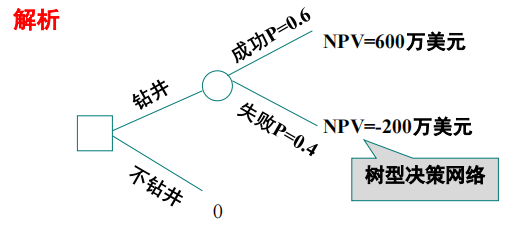
\includegraphics[width=\linewidth]{image/决策树.png}
\end{figure}

某勘探项目面临如下决策:是否购买区块?购买后,是直接钻井,还是先进行地震勘探?如果第一口井是干井,是否钻第二口井?

\noindent \textbf{基础资料}
\noindent \textbf{(1)成本收益数据}
大发现的价值=\$40

小发现的价值=\$15

区块购买成本=\$3

钻井成本=\$1

地震勘探成本=\$2

\noindent \textbf{(2)概率数据}
\textbf{直接钻井情况下(若第一口井为干井,才考虑是否钻第二口井。)}

大发现:第一口井概率5\%,第二口井概率7.5\%;

小发现:第一口井概率5\%,第二口井概率7.5\%;

干井:第一口井概率90\%,第二口井概率为85\%。

\textbf{先进行地震勘探后再钻井情况下地震勘探后发现有潜在油藏的概率为50\%,若第一口井为干井,才考虑是否钻第二口井。}

大发现:第一口井概率15\%,第二口井概率20\%;

小发现:第一口井概率15\%,第二口井概率20\%;

干井:第一口井概率70\%,第二口井概率为60\%。

\begin{figure}[H]
    \centering
    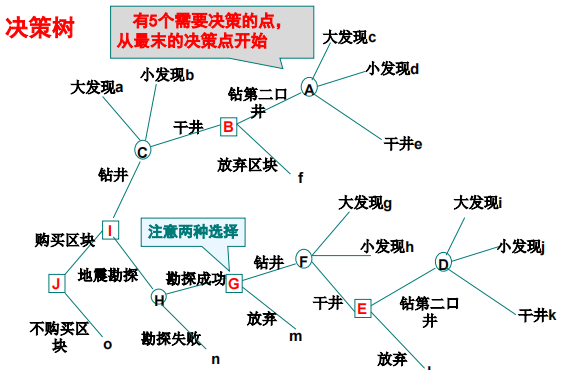
\includegraphics[width=1\linewidth]{image/决策树1-例1.png}
\end{figure}

\begin{figure}[H]
    \centering
    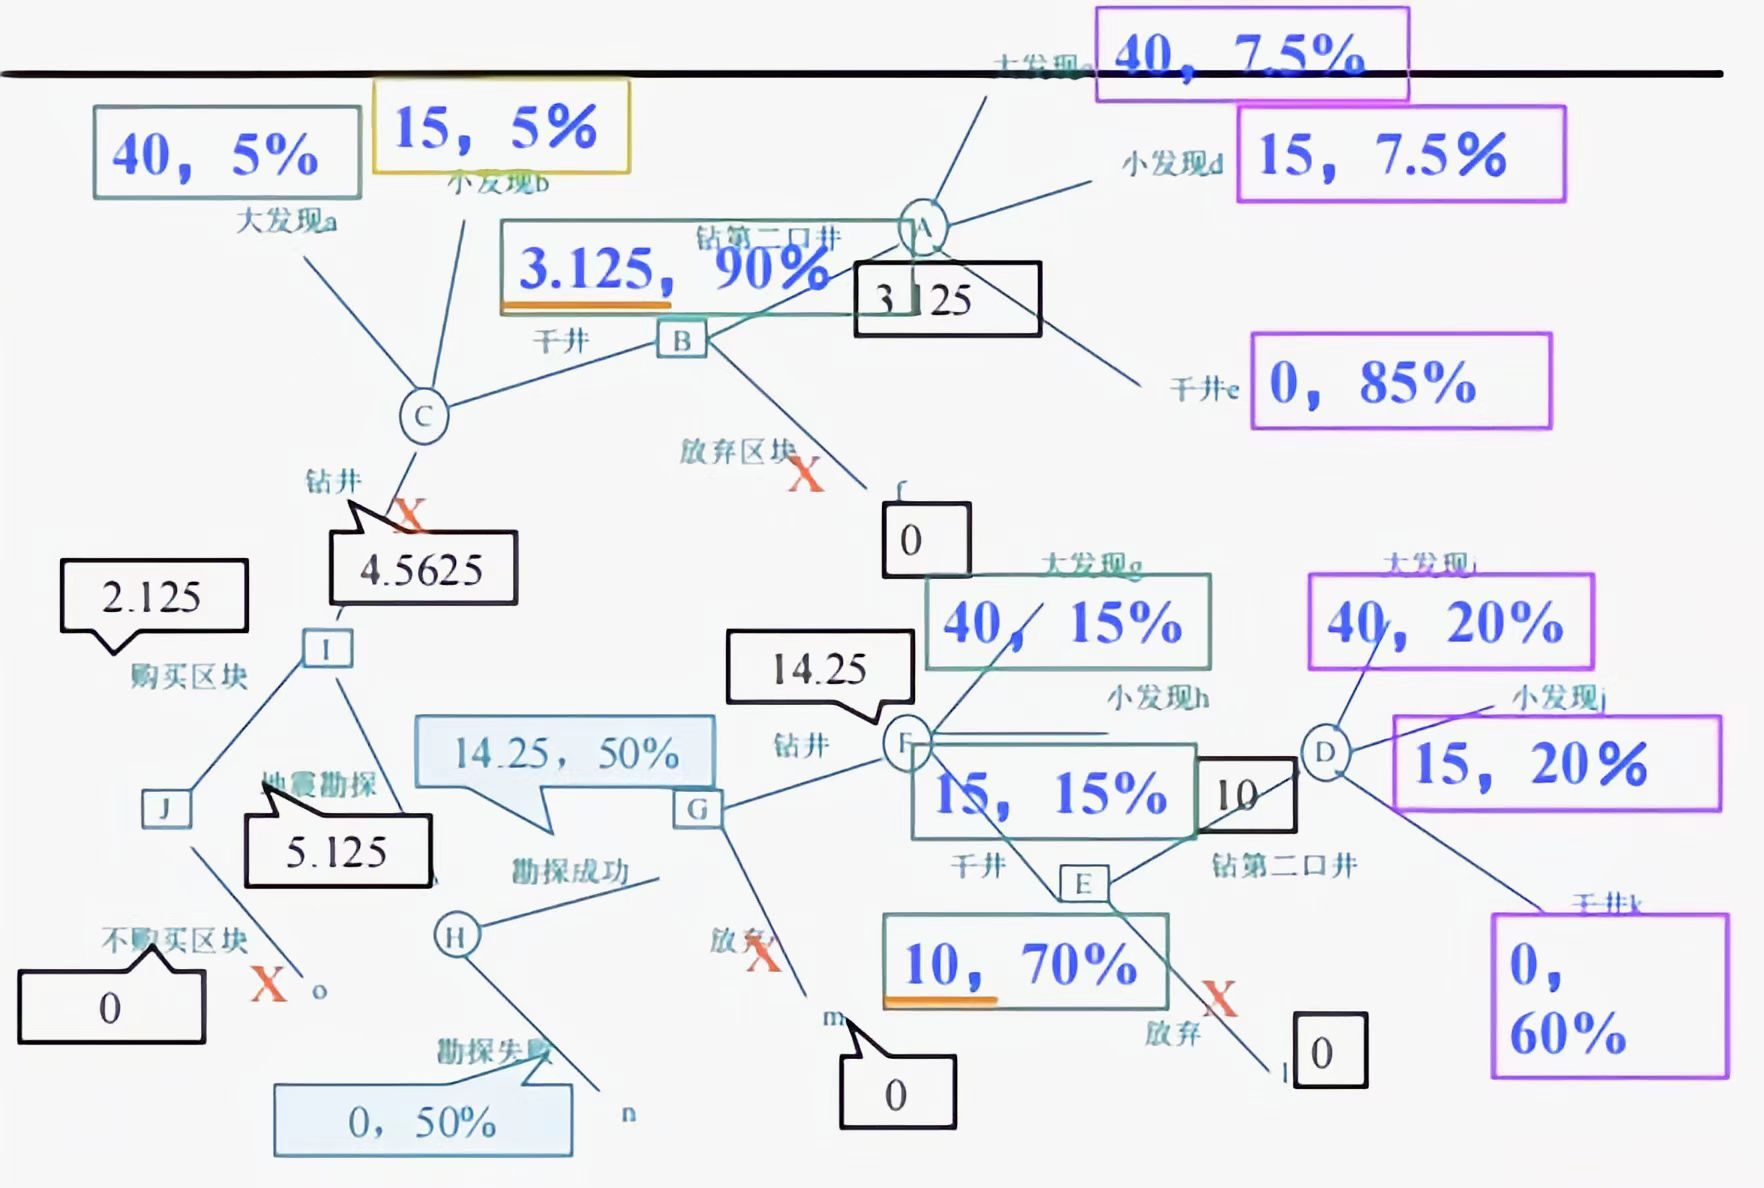
\includegraphics[width=1\linewidth]{image/决策树2-例1.jpg}
\end{figure}

\noindent \textbf{解析:}

利用决策树进行多阶段风险决策,要从最末一级决策点开始。

\textbf{(1)决策点B}

状态点A的期望净现值:

$ENPV_A=-\$1+(\$40×0.075+\$15×0.075+\$0×0.85)=\$3.125$

与放弃(净现值为零)相比,应该决策钻第二口井。

\textbf{(2)决策点E}

状态点D的期望净现值:

$ENPV_D=-\$1+(\$40×0.20+\$15×0.20+\$0×0.60)=\$10$

与放弃(净现值为零)相比,应该决策钻第二口井。

\textbf{(3)决策点G}

状态点F的期望净现值:

$ENPV_F=-\$1+(\$40×0.15+\$15×0.15+\$10×0.70)=\$14.25$

(注意:用状态D的期望净现值代替E决策点)

与放弃(净现值为零)相比,应该决策钻第一口井。

\textbf{(4)决策点I}

状态点C的期望净现值:

$ENPV_C=-\$1+(\$40×0.05+\$15×0.05+\$3.125×0.90)=\$4.5625$

状态点H的期望净现值:

$ENPV_H=-\$2+(\$14.25×0.50+\$0×0.50)
=\$5.125$

状态点C与状态点H相比,应该选择地震勘探。

\textbf{(5)决策点J}

购买区块的期望净现值$=-\$3+\$5.125=\$2.125$

与不购买(净现值为零)相比,应该选择购买。

\textbf{(6)决策结论}

通过决策树分析,决策结果如下:

购买区块;先进行地震勘探;如果勘探成功,钻第一口井;如果第一口井是干井,继续钻第二口井。

\begin{figure}[H]
    \centering
    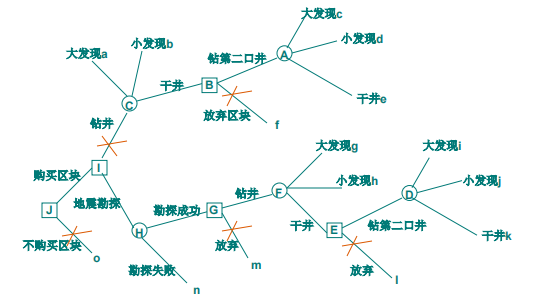
\includegraphics[width=1\linewidth]{image/决策结果.png}
\end{figure}
\chapter{项目的财务评价}
\section{财务评价概述}
\subsection{财务评价的概念}
财务评价是根据国家现行的财税制度和价格体系,在财务效益与费用的估算以及编制财务辅助报表的基础上,\textbf{编制财务报表,计算财务分析指标,考察和分析项目的盈利能力、偿债能力和财务生存能力,判断项目的财务可行性},明确项目对财务主体的价值以及对投资者的贡献,为投资决策、融资决策以及银行贷款等提供依据。

  ——2006年国家发改委和建设部联合发布的《建设项目经济评价方法与参数》(第三版)

\subsection{财务评价的内容和步骤}
(1)选取财务评价基础数据与参数。

(2)估算财务效益与费用,形成财务评价辅助报表,编制资金规划与计划。

(3)编制财务评价的基本报表。

(4)根据融资前分析和融资后分析的要求,计算评价指标,进行盈利能力分析、偿债能力分析、财务生存能力分析等。

(5)不确定性分析和风险分析。

(6)形成财务评价结论。

\section{财务效益与费用估算}
\subsection{财务效益估算}
财务效益主要包括营业收入,项目得到的各种补贴、项目寿命期末回收的固定资产余值和流动资金。

营业收入包括销售产品或提供服务所获得的收入,其估算的基础数据,包括产品或服务的数量和价格。

对于生产多种产品和提供多项服务的,应分别估算各种产品及服务的营业收入。

\begin{figure}[H]
    \centering
    \includegraphics[width=1\linewidth]{image/营业收入、营业税金及附加和增值税估算表.png}
    \caption{营业收入、营业税金及附加和增值税估算表}
\end{figure}

\subsection{投资的估算}

\subsubsection{1. 建设投资估算}

\textbf{简单估算法、概算法、形成资产法}

项目规划和建议书阶段,投资估算要求精度低,可利用简单估算法。

单位生产能力法、生产能力指数法、系数估算法。

\noindent \textbf{A 单位生产能力法——简单估算法}

依据调查的统计资料,利用相近规模的单位生产能力投资乘以建设规模,即得拟建项目投资。

$$C_2=(\frac{C_1}{Q_1})Q_2f$$

式中,C1:已建类似项目的投资额;C2:拟建项目投资额;Q1:已建类似项目的生产能力;Q2:拟建项目的生产能力;f:不同时期、不同地点的定额、单价、费用变更等的综合调整系数。

\textbf{例:}假定某地拟建一座2000套客房的豪华旅馆,另有一座某豪华旅馆最近在该地竣工,且掌握了以下资料:它有2500套客房,有门厅、餐厅、会议室、游泳池、夜总会、网球场等设施。总造价为10250万美元。估算新建项目的总投资。

\textbf{解:}折算为每套客房的造价:4.1万美元

同一个地方,且各方面有可比性的具有2000套客房的豪华旅馆造价估算值为:4.1万美元×2000=8200万美元。

\noindent \textbf{B 生产能力指数法——简单估算法}

又称指数估算法,它是根据已建成的类似项目生产能力和投资额来粗略估算拟建项目投资额的方法,是对单位生产能力估算法的改进。
$$C_2=C_1(\frac{Q_2}{Q_1})^x \cdot f$$
式中:x—生产能力指数。正常情况下,$0 \leq x \leq 1$。

造价与规模(或容量)呈非线性关系,且单位造价随工程规模(或容量)的增大而减小。

\noindent \textbf{C 系数估算法——简单估算法}

以某个装置或某项设备费为基数,乘以适当系数来推算项目的建设费用。这种方法比较简单,但没有考虑设备规格、材质的差异,所以精确度不高。

总建设费用=主要设备费(1+管线、仪表、建筑等费用估算系数)*(1+间接费总估算系数)

\noindent \textbf{概算法和形成资产法}

按照费用的归集方式有概算法和形成资产法。

\textbf{概算法。}把建设项目划分为建筑工程费、设备购置费、安装工程费用及工程建设其他费用等费用项目或单位工程,再根据各种具体的投资估算指标,进行各项费用项目或单位工程投资的估算,在此基础上,可汇总成每一单项工程的投资。另外再估算工程建设其他费用及预备费,即求得项目建设总投资。

\textbf{形成资产法。}由形成固定资产的费用、形成无形资产的费用、形成其他资产的费用和预备费用四部分组成。

\noindent \textbf{建设投资的概算法}

\textbf{基本预备费估算:}是指在项目实施中可能发生难以预料的支出,需要事先预留的费用,又称工程不可预见费,主要指设计变更及施工过程中可能增加工程量的费用。基本预备费以建筑工程费、设备购置费、安装工程费及工程建设其他费用之和为计算基数乘以基本预备费率计算。

中石化:

(固定资产+无形资产+其他资产)$\times $不可预见费率

10\%-12\%,适用于综合类及国内无同类装置项目

8\%-10\%,适用于国内已见有同类装置项目。

\textbf{涨价预备费估算:}涨价预备费是对建设工期较长的项目,由于在建设期内可发生材料、设备、人工等价格上涨引起投资增加,需要事先预留的费用,也称价格变动不可预见费。涨价预备费以建筑工程费、设备购置费、安装工程费之和为计算基础。计算公式为:

$$PC=\sum_{i=1}^{n}I_t[(1+f)^t-1]$$

其中:PC—涨价预备费;$I_t$—第t年的建筑工程费、设备购置费和安装工程费之和;f—建设期价格上涨指数;n—建设期。

\subsubsection{2. 流动资金估算}

扩大指标估算法:是参照同类企业流动资金占营业收入或经营成本的比例、或者单位产量占用营运资金的数额估算流动资金。

在项目建议书阶段一般可采用扩大指标估算法。

流动资金=年营业收入额×营业收入资金率

流动资金=年经营成本×经营成本资金率

中石化石油天然气项目经营成本资金率:15\%-25\%

流动资金=年产量×单位产量占用流动资金额

\subsubsection{3. 建设期利息的估算}

建设期利息包括银行借款和其他债务资金的利息,以及其他融资费用。
其他融资费用是指某些债务融资中发生的手续费、承诺费、管理费、信贷保险费等融资费用。

通常假定借款均在每年的年中支用,借款当年按半年计算,其余各年份按全年计息。

各年应计利息=(年初借款本金累计+本年借款额/2)$\times $年利率

\subsection{总成本费用的估算}

\subsubsection{1. 生产成本加期间费用估算法}

即总成本费用=生产成本+期间费用

生产成本=直接材料费+直接燃料和动力费+直接工资+其他直接支出+制造费用

期间费用=管理费用+营业费用+财务费用

\subsubsection{2. 生产要素估算法}

总成本费用=外购原材料、燃料和动力费+工资及福利费+折旧费+摊销费+修理费+利息支出+其他费用

\subsection{经营成本的估算}

经营成本=外购原材料、燃料和动力费+工资及福利费+修理费+其他费用

如果以会计核算中的总成本费用为基础,则是在总成本费用中要扣除虽计入产品的成本费用中,但实际并没有发生现金支出的费用项目。

经营成本=总成本费用-折旧费-摊销费-利息支出

\subsection{税费的估算}

\textbf{增值税。}当采用含税价格计算销售收入和原材料、燃料动力成本时,利润和利润分配表以及现金流量表中应单列增值税科目;采用不含税价格计算时,利润和利润分配表以及现金流量表中不包含增值税科目。

\textbf{消费税。}我国对部分货物征收消费税。项目评价中对适用消费税的产品,应按税法规定计算消费税。

\textbf{土地增值税。}是按转让房地产取得的增值额征收的税种。房地产开发项目应按规定计算土地增值税。

\textbf{资源税。}是国家队开采特定矿产品或生产盐的单位和个人征收的税种。通常按矿产的产量计征。

在会计处理上,消费税、土地增值税、资源税和城建税、教育费附加均可包含在营业税金及附加中。税金及附加应作为利润和利润分配表中的科目。

\subsection{维持运营投资}

某些项目在运营期需要投入一定的固定资产投资才能得以维持正常运营,例如设备更新费用、矿山的井巷开拓延伸费用等。发生维持运营投资时应将其列入现金流量表作为现金流出,参与内部收益率的计算。同时,也应反映在财务计划现金流量表中,参与财务生存能力分析。

如煤炭项目,为维持正常生产,在生产期内需要投入一定的固定资产或费用,包括固定资产更新投资、安全生产投入、维简费开支的其他维持简单再生产投入、开拓延深费和追加投资等,这些维持运营投资,应在现金流量表中将其作为现金流出。

固定资产更新投资、开拓延深费和追加投资应予以资本化,安全生产投入、维检费开支等其他维持简单再生产投入应予以费用化。

\begin{figure}[H]
    \centering
    \includegraphics[width=\linewidth]{image/财务分析辅助报表关系图.png}
    \caption{财务分析辅助报表关系图}
\end{figure}

\section{财务评价的基本报表}

\noindent 复习要点:\\
\textbf{现金流量表 重点}\\
\textbf{1. 项目投资现金流量表 最重要}\\
\textbf{2. 项目资本金现金流量表 次重要}\\
\textbf{3. 投资各方现金流量表}\\
利润与利润分配表\\
财务计划现金流量表\\
借款还本付息计划表

\subsection{现金流量表}
\subsubsection{1.项目投资现金流量表(要求会编制)}
是以项目作为一个独立系统,不区分项目资金的来源,反映项目在整个计算期内的现金流入和现金流出,反映项目投资的盈利能力,用于计算项目投资内部收益率及净现值等财务分析指标。

其现金流量的计算与成本核算的算法不同,现金流量计算中只体现现金收支,不体现非现金的摊派(如折旧、摊销)等。

\begin{figure}[H]
    \centering
    \includegraphics[width=0.6\linewidth]{image/项目投资现金流量表1.png}
    \caption{项目投资现金流量表}
\end{figure}

\subsubsection{2. 项目资本金现金流量表(不太重要)}
从项目法人(或投资者整体)角度出发,以项目资本金作为计算的基础,把借款本金偿还和利息支付作为现金流出,用以计算资本金内部收益率,反映投资者权益投资的获利能力。对资本金只计算税后净现金流量,因为税前净现金流量没有实际价值。

\begin{figure}[H]
    \centering
    \includegraphics[width=0.6\linewidth]{image/项目资本金现金流量表.png}
    \caption{项目资本金现金流量表}
\end{figure}

\subsubsection{3. 投资各方现金流量表(自学)}
分别从各个投资者的角度出发,以投资者的出资额作为计算的基础,用于计算投资各方内部收益率。

\begin{figure}[H]
    \centering
    \includegraphics[width=0.6\linewidth]{image/投资各方现金流量表.png}
    \caption{投资各方现金流量表}
\end{figure}

\subsection{利润与利润分配表}
反映项目计算期内各年营业收入、总成本费用、利润总额等情况,以及所得税后利润的分配,用于计算总投资收益率、项目资本金净利润率等指标。

要求:会进行简单的利润计算。

利润=收入-总成本费用-营业税金及附加

掌握总成本费用与经营成本之间的区别与联系。

\begin{figure}[H]
    \centering
    \includegraphics[width=0.6\linewidth]{image/利润与利润分配表.png}
    \caption{利润与利润分配表}
\end{figure}

\subsection{财务计划现金流量表(了解)}
反映项目计算期各年的投资、融资及经营活动的现金流入和流出,用于计算累计盈余资金,分析项目是否有足够的净现金流量维持正常运营,以实现财务可持续性,体现项目的财务生存能力。

\begin{figure}[H]
    \centering
    \includegraphics[width=0.6\linewidth]{image/财务计划现金流量表.png}
    \caption{财务计划现金流量表}
\end{figure}

\begin{figure}[H]
    \centering
    \includegraphics[width=0.6\linewidth]{image/财务计划现金流量表(续).png}
    \caption{财务计划现金流量表(续)}
\end{figure}

\section{财务评价的指标体系}
\subsection{盈利能力分析指标体系}
财务净现值、财务内部收益率、资本金财务内部收益率、投资各方财务内部收益率、项目动态投资回收期、总投资收益率、项目资本金净利润率、投资回收期。

\subsection{偿债能力指标体系}
\subsubsection{1. 利息备付率}
利息备付率= 税息前利润 / 当期应付利息 $\times$ 100\%

税息前利润=利润总额+计入总成本费用的利息费用;

当期应付利息—计入总成本费用中的应付利息。

利息备付率应分年计算,利息备付率高,表明利息偿付的保障程度高。

利息备付率应大于1,并结合债权人的要求确定。

\subsubsection{2. 偿债备付率}
偿债备付率=可用于还本付息的资金/当期应还本付息的金额 $\times $100\%

可用于还本付息的资金—包括可用于还款的折旧和摊销、成本中列支的利息费用、可用于还款的利润等,也即息税前利润加折旧和摊销,并减去所得税;

应还本付息的金额—包括还本金额和计入总成本费用的全部利息。

偿债备付率应分年计算,偿债备付率高,表明可用于还本付息的资金保障程度高。

偿债备付率应大于1,并结合债权人的要求确定。

\subsubsection{3. 资产负债率}
资产负债率= 期末负债总额 / 期末资产总额 $\times $ 100\%

适度的资产负债率,表明企业经营安全、稳健,具有较强的筹资能力,也表明企业和债权人的风险较小。对该指标的分析,应结合国家宏观经济状况、行业发展趋势、企业所处竞争环境等具体条件判定。项目财务分析中,在长期债务还清后,可不再计算资产负债率。

\subsection{财务生存能力分析}
财务生存能力分析也称为资金平衡分析

拥有足够的经营净现金流量是财务可持续性的基本条件,特别是在运营初期。

各年累计盈余资金不出现负值是财务生存的必要条件。

\begin{figure}[H]
    \centering
    \includegraphics[width=0.6\linewidth]{image/财务分析和评价指标与基本财务报表的对应关系.png}
    \caption{财务分析和评价指标与基本财务报表的对应关系}
\end{figure}

\textbf{举例(重要,理解并掌握):}某项目总投资1350万元,其中固定资产投资1000万元,流动资金350万元,于项目第一年年初投入。项目当年建成投产,生产期10年,每年产品销售收入800万元,年经营成本400万元,年营业税金及附加80万元。固定资产投资全部形成固定资产原值,在生产期采用直线折旧法进行折旧,折旧年限为10年,净残值率为5\%。设所得税税率为40\%。

\begin{figure}[H]
    \centering
    \includegraphics[width=0.6\linewidth]{image/项目投资现金流量表2.png}
\end{figure}

\textbf{例(续):}上述项目中固定资产投资中50\%是长期借款,年利率8\%,借款本金从生产期开始分10年等额偿还,每年支付未偿还借款的利息;流动资金投资的40\%来自借款,借款利率为5\%,第10年末一次偿还流动资金借款,每年支付相应利息。

\begin{figure}[H]
    \centering
    \includegraphics[width=0.75\linewidth]{image/生存能力分析1.png}
\end{figure}

\begin{figure}[H]
    \centering
    \includegraphics[width=0.75\linewidth]{image/生存能力分析2.png}
\end{figure}

\begin{figure}[H]
    \centering
    \includegraphics[width=0.75\linewidth]{image/生存能力分析3.png}
\end{figure}

\begin{figure}[H]
    \centering
    \includegraphics[width=0.75\linewidth]{image/生存能力分析4.png}
\end{figure}

\begin{figure}[H]
    \centering
    \includegraphics[width=0.75\linewidth]{image/生存能力分析5.png}
\end{figure}
\chapter{考试分析}
按照老师给的考试题型,选择 15 个,共 30 分;判断 10 个,共 15 分;简答:2 个,共 12 分;计算分析:共 43 分。

绪论(即第一章)重点不多,考点也仅有几个,已经在文档中标出;第二、第三章是考核重点,这两章在期末中大概占50\%的考试内容;第四、第五章大概占30\%到40\%;因为第六章最难,所以第六章主要以大小案例形式出现,占总分的15分,期末考试不会出计算分析题,可能会有10到20分的简答和选择判断。


\end{document}
